% !TeX root = sablona-prace.tex

% Soubory musí být v kódování, které je nastaveno v příkazu \usepackage[...]{inputenc}

\documentclass[%        Základní nastavení
%  draft,    				  % Testovací překlad
  12pt,       				% Velikost základního písma je 12 bodů
  a4paper,    				% Formát papíru je A4
  %oneside,      			% Jednostranný tisk
	twoside,      			% Dvoustranný tisk (kapitoly a další důležité části tedy začínají na lichých stranách)
	unicode,						% Záložky a metainformace ve výsledném  PDF budou v kódování unicode
]{report}				    	% Dokument třídy 'zpráva', vhodná pro sazbu závěrečných prací s kapitolami

\usepackage[utf8]		  %	Kódování zdrojových souborů je UTF-8
	{inputenc}					% Balíček pro nastavení kódování zdrojových souborů

\usepackage[				% Nastavení geometrie stránky
	bindingoffset=10mm,		% Hřbet pro vazbu
	hmargin={25mm,25mm},	% Vnitřní a vnější okraj
	vmargin={25mm,34mm},	% Horní a dolní okraj
	footskip=17mm,			  % Velikost zápatí
	nohead,					      % Bez záhlaví
	marginparsep=2mm,		  % Vzdálenost marginálií
	marginparwidth=18mm,	% Šířka marginálií
]{geometry}

\usepackage{sectsty}
	%přetypuje nadpisy všech úrovní na bezpatkové, kromě \chapter, která je přenastavena zvlášť v thesis.sty
	\allsectionsfont{\sffamily}

\usepackage{graphicx} % Balíček 'graphicx' pro vkládání obrázků
											% Nutné pro vložení logotypů školy a fakulty

\usepackage[          % Balíček 'acronym' pro sazby zkratek a symbolů
	nohyperlinks				% Nebudou tvořeny hypertextové odkazy do seznamu zkratek
]{acronym}						
											% Nutné pro použití prostředí 'acronym' balíčku 'thesis'

\usepackage[
	breaklinks=true,		% Hypertextové odkazy mohou obsahovat zalomení řádku
	hypertexnames=false % Názvy hypertext. odkazů budou tvořeny nezávisle na názvech TeXu
]{hyperref}						% Balíček 'hyperref' pro sazbu hypertextových odkazů
											% Nutné pro použití příkazu 'pdfsettings' balíčku 'thesis'

\usepackage{pdfpages} % Balíček umožňující vkládat stránky z PDF souborů
                      % Nutné při vkládání titulních listů a zadání přímo
                      % ve formátu PDF z informačního systému

\usepackage{enumitem} % Balíček pro nastavení mezerování v odrážkách
  \setlist{topsep=0pt,partopsep=0pt,noitemsep} % konkrétní nastavení

\usepackage{cmap} 		% Balíček cmap zajišťuje, že PDF vytvořené `pdflatexem' je
											% plně "prohledávatelné" a "kopírovatelné"

%\usepackage{upgreek}	% Balíček pro sazbu stojatých řeckých písmem
											%% např. stojaté pí: \uppi
											%% např. stojaté mí: \upmu (použitelné třeba v mikrometrech)
											%% pozor, grafická nekompatibilita s fonty typu Computer Modern!
                      
%\usepackage{amsmath} %balíček pro sabu náročnější matematiky                 

\usepackage{dirtree}	% sazba adresářové struktury
                      % vhodné pro prezentaci obsahu elektronické přílohy (např. CD)

\usepackage[formats]{listings}	% Balíček pro sazbu zdrojových textů
\lstset{              % nastavení
%	Definice jazyka použitého ve výpisech
%    language=[LaTeX]{TeX},	% LaTeX
%	language={Matlab},		% Matlab
	language={C},           % jazyk C
    basicstyle=\ttfamily,	% definice základního stylu písma
    tabsize=2,			% definice velikosti tabulátoru
    inputencoding=utf8,         % pro soubory uložené v kódování UTF-8
		columns=fixed,  %fixed nebo flexible,
		fontadjust=true %licovani sloupcu
    extendedchars=true,
    literate=%  definice symbolů s diakritikou
    {á}{{\'a}}1
    {č}{{\v{c}}}1
    {ď}{{\v{d}}}1
    {é}{{\'e}}1
    {ě}{{\v{e}}}1
    {í}{{\'i}}1
    {ň}{{\v{n}}}1
    {ó}{{\'o}}1
    {ř}{{\v{r}}}1
    {š}{{\v{s}}}1
    {ť}{{\v{t}}}1
    {ú}{{\'u}}1
    {ů}{{\r{u}}}1
    {ý}{{\'y}}1
    {ž}{{\v{z}}}1
    {Á}{{\'A}}1
    {Č}{{\v{C}}}1
    {Ď}{{\v{D}}}1
    {É}{{\'E}}1
    {Ě}{{\v{E}}}1
    {Í}{{\'I}}1
    {Ň}{{\v{N}}}1
    {Ó}{{\'O}}1
    {Ř}{{\v{R}}}1
    {Š}{{\v{S}}}1
    {Ť}{{\v{T}}}1
    {Ú}{{\'U}}1
    {Ů}{{\r{U}}}1
    {Ý}{{\'Y}}1
    {Ž}{{\v{Z}}}1
}

%%%%%%%%%%%%%%%%%%%%%%%%%%%%%%%%%%%%%%%%%%%%%%%%%%%%%%%%%%%%%%%%%
%%%%%%      Definice informací o dokumentu             %%%%%%%%%%
%%%%%%%%%%%%%%%%%%%%%%%%%%%%%%%%%%%%%%%%%%%%%%%%%%%%%%%%%%%%%%%%%

% V tomto souboru se nastavují téměř veškeré informace, proměnné mezi studenty:
% jméno, název práce, pohlaví atd.
% Tento soubor je SDÍLENÝ mezi textem práce a prezentací k obhajobě -- netřeba něco nastavovat na dvou místech.

\usepackage[
%%% Z následujících voleb jazyka lze použít pouze jednu
  czech-english,		% originální jazyk je čeština, překlad je anglicky (výchozí)
  %english-czech,	% originální jazyk je angličtina, překlad je česky
  %slovak-english,	% originální jazyk je slovenština, překlad je anglicky
  %english-slovak,	% originální jazyk je angličtina, překlad je slovensky
%
%%% Z následujících voleb typu práce lze použít pouze jednu
  %semestral,		  % semestrální práce (nesází se abstrakty, prohlášení, poděkování) (výchozí)
  bachelor,			%	bakalářská práce
  %master,			  % diplomová práce
  %treatise,			% pojednání o disertační práci
  %doctoral,			% disertační práce
%
%%% Z následujících voleb zarovnání objektů lze použít pouze jednu
%  left,				  % rovnice a popisky plovoucích objektů budou zarovnány vlevo
	center,			    % rovnice a popisky plovoucích objektů budou zarovnány na střed (vychozi)
%
]{thesis}   % Balíček pro sazbu studentských prací


%%% Jméno a příjmení autora ve tvaru
%  [tituly před jménem]{Křestní}{Příjmení}[tituly za jménem]
% Pokud osoba nemá titul před/za jménem, smažte celý řetězec '[...]'
\author{Martin}{Kousal}

%%% Identifikační číslo autora (VUT ID)
\butid{221063}

%%% Pohlaví autora/autorky
% (nepoužije se ve variantě english-czech ani english-slovak)
% Číselná hodnota: 1...žena, 0...muž
\gender{0}

%%% Jméno a příjmení vedoucího/školitele včetně titulů
%  [tituly před jménem]{Křestní}{Příjmení}[tituly za jménem]
% Pokud osoba nemá titul před/za jménem, smažte celý řetězec '[...]'
\advisor[doc. Ing.]{Tomáš}{Frýza}[Ph.D.]

%%% Jméno a příjmení oponenta včetně titulů
%  [tituly před jménem]{Křestní}{Příjmení}[tituly za jménem]
% Pokud osoba nemá titul před/za jménem, smažte celý řetězec '[...]'
% Nastavení oponenta se uplatní pouze v prezentaci k obhajobě;
% v případě, že nechcete, aby se na titulním snímku prezentace zobrazoval oponent, pouze příkaz zakomentujte;
% u obhajoby semestrální práce se oponent nezobrazuje (jelikož neexistuje)
% U dizertační práce jsou typicky dva až tři oponenti. Pokud je chcete mít na titulním slajdu, prosím ručně odkomentujte a upravte jejich jména v definici "VUT title page" v souboru thesis.sty.
\opponent[doc.\ Mgr.]{Křestní}{Příjmení}[Ph.D.]

%%% Název práce
%  Parametr ve složených závorkách {} je název v originálním jazyce,
%  parametr v hranatých závorkách [] je překlad (podle toho jaký je originální jazyk).
%  V případě, že název Vaší práce je dlouhý a nevleze se celý do zápatí prezentace, použijte příkaz
%  \def\insertshorttitle{Zkác.\ náz.\ práce}
%  kde jako parametr vyplníte zkrácený název. Pokud nechcete zkracovat název, budete muset předefinovat,
%  jak se vytváří patička slidu. Viz odkaz: https://bit.ly/3EJTp5A
\title[IoT air monitoring]{IoT monitoring ovzduší}

%%% Označení oboru studia
%  Parametr ve složených závorkách {} je název oboru v originálním jazyce,
%  parametr v hranatých závorkách [] je překlad
\specialization[Electronics and Communication Technologies]{Elektronika a komunikační technologie}

%%% Označení ústavu
%  Parametr ve složených závorkách {} je název ústavu v originálním jazyce,
%  parametr v hranatých závorkách [] je překlad
%\department[Department of Control and Instrumentation]{Ústav automatizace a měřicí techniky}
%\department[Department of Biomedical Engineering]{Ústav biomedicínského inženýrství}
%\department[Department of Electrical Power Engineering]{Ústav elektroenergetiky}
%\department[Department of Electrical and Electronic Technology]{Ústav elektrotechnologie}
%\department[Department of Physics]{Ústav fyziky}
%\department[Department of Foreign Languages]{Ústav jazyků}
%\department[Department of Mathematics]{Ústav matematiky}
%\department[Department of Microelectronics]{Ústav mikroelektroniky}
\department[Department of Radio Electronics]{Ústav radioelektroniky}
%\department[Department of Theoretical and Experimental Electrical Engineering]{Ústav teoretické a experimentální elektrotechniky}
%\department[Department of Telecommunications]{Ústav telekomunikací}
%\department[Department of Power Electrical and Electronic Engineering]{Ústav výkonové elektrotechniky a elektroniky}

%%% Označení fakulty
%  Parametr ve složených závorkách {} je název fakulty v originálním jazyce,
%  parametr v hranatých závorkách [] je překlad
%\faculty[Faculty of Architecture]{Fakulta architektury}
\faculty[Faculty of Electrical Engineering and~Communication]{Fakulta elektrotechniky a~komunikačních technologií}
%\faculty[Faculty of Chemistry]{Fakulta chemická}
%\faculty[Faculty of Information Technology]{Fakulta informačních technologií}
%\faculty[Faculty of Business and Management]{Fakulta podnikatelská}
%\faculty[Faculty of Civil Engineering]{Fakulta stavební}
%\faculty[Faculty of Mechanical Engineering]{Fakulta strojního inženýrství}
%\faculty[Faculty of Fine Arts]{Fakulta výtvarných umění}
%
%Nastavení logotypu (v hranatych zavorkach zkracene logo, ve slozenych plne):
\facultylogo[logo/FEKT_zkratka_barevne_PANTONE_CZ]{logo/logo_fekt_urel_cze}

%%% Rok odevzdání práce
\graduateyear{2022}
%%% Akademický rok odevzdání práce
\academicyear{2021/22}

%%% Datum obhajoby (uplatní se pouze v prezentaci k obhajobě)
\date{7.\,1.\,2022}

%%% Místo obhajoby
% Na titulních stránkách bude automaticky vysázeno VELKÝMI písmeny (pokud tyto stránky sází šablona)
\city{Brno}

%%% Abstrakt
\abstract[%
The purpose of this bachelor work is to make a device that can measure air quality parameters and send them wirelessly to the server, where that measured data are processed and then shown to the user. The aim is to create a device with the lowest possible power consumption for the possibility of battery operation.
]{%
Tato bakalářská práce se zabývá vytvořením zařízení pro měření kvalitativních parametrů ovzduší a které je následně bezdrátově přenáší na server, kde se naměřená data zpracovávají a zobrazují uživateli. Cílem je vytvořit zařízení s co nejnižším odběrem pro možnost provozu na akumulátor.
}

%%% Klíčová slova
\keywrds[%
IoT, ESP32, sensors, dust particles sensor, air quality, LoRa, gas sensor, temperature, humidity, light intensity, UV light
]{%
IoT, ESP32, senzory, senzor prachových částic, kvalita vzduchu, LoRa, senzor plynů, teplota, vlhkost, intenzita osvětlení, UV záření
}

%%% Poděkování
\acknowledgement{%
Rád bych poděkoval vedoucímu bakalářské práce
panu doc.~Ing.~Tomáši Frýzovi, Ph.D.\ za odborné vedení,
konzultace, trpělivost a~podnětné návrhy k~práci.
}%  % do tohoto souboru doplňte údaje o sobě, druhu práce, názvu...

%%%%%%%%%%%%%%%%%%%%%%%%%%%%%%%%%%%%%%%%%%%%%%%%%%%%%%%%%%%%%%%%%%%%%%%%

%%%%%%%%%%%%%%%%%%%%%%%%%%%%%%%%%%%%%%%%%%%%%%%%%%%%%%%%%%%%%%%%%%%%%%%%
%%%%%%     Nastavení polí ve Vlastnostech dokumentu PDF      %%%%%%%%%%%
%%%%%%%%%%%%%%%%%%%%%%%%%%%%%%%%%%%%%%%%%%%%%%%%%%%%%%%%%%%%%%%%%%%%%%%%
%% Při načteném balíčku 'hyperref' lze použít příkaz '\pdfsettings':
\pdfsettings
%  Nastavení polí je možné provést také ručně příkazem:
%\hypersetup{
%  pdftitle={Název studentské práce},    	% Pole 'Document Title'
%  pdfauthor={Autor studenstké práce},   	% Pole 'Author'
%  pdfsubject={Typ práce}, 						  	% Pole 'Subject'
%  pdfkeywords={Klíčová slova}           	% Pole 'Keywords'
%}
%%%%%%%%%%%%%%%%%%%%%%%%%%%%%%%%%%%%%%%%%%%%%%%%%%%%%%%%%%%%%%%%%%%%%%%

\pdfmapfile{=vafle.map}

%%%%%%%%%%%%%%%%%%%%%%%%%%%%%%%%%%%%%%%%%%%%%%%%%%%%%%%%%%%%%%%%%%%%%%%
%%%%%%%%%%%       Začátek dokumentu               %%%%%%%%%%%%%%%%%%%%%
%%%%%%%%%%%%%%%%%%%%%%%%%%%%%%%%%%%%%%%%%%%%%%%%%%%%%%%%%%%%%%%%%%%%%%%
\begin{document}
\pagestyle{empty} %vypnutí číslování stránek

%%% Vložení desek -- od září 2021 na žádost fakulty nepoužíváno
%\includepdf[pages=1]%  buďto generovaných informačním systémem
  %{pdf/student-desky}% název souboru nesmí obsahovat mezery!
%%% NEBO vytvoření desek z balíčku
%%\makecover
%%%
%\oddpage % při dvojstranném tisku přidá prázdnou stránku
%% kazdopádně ale:
%\setcounter{page}{1} %resetovaní čítače stránek -- desky do číslování nezahrnujeme

%% Vložení titulního listu
\includepdf[pages=1]%    buďto generovaného informačním systémem
  {pdf/student-titulka}% název souboru nesmí obsahovat mezery!
%% NEBO vytvoření titulní stránky z balíčku
%\maketitle
%%
\oddpage  % při dvojstranném tisku se přidá prázdná stránka
   
%% Vložení zadání
\includepdf[pages=1]%   buďto generovaného informačním systémem
  {pdf/student-zadani}% název souboru nesmí obsahovat mezery!
%% NEBO lze vytvořit prázdný list příkazem ze šablony
%\patternpage{}%
%	{\sffamily\Huge\centering ZDE VLOŽIT LIST ZADÁNÍ}%
%	{\sffamily\centering Z~důvodu správného číslování stránek}
%%
\oddpage% při dvojstranném tisku se přidá prázdná stránka

%% Vysázení stránky s abstraktem
\makeabstract

% Vysázení stránky s rozšířeným abstraktem
% (pokud píšete práci v češtině či slovenštině, vložení rozšířeného abstraktu zrušte;
%  pro semestrální projekt také není potřeba rozšířený abstrakt uvádět)
% Vysázení stránky s rozšířeným abstraktem
% (týká se pouze bc. a dp. prací psaných v angličtině, viz Směrnice rektora 72/2017)
\cleardoublepage
\noindent
{\large\sffamily\bfseries\MakeUppercase{Rozšířený abstrakt}}
\\
Výtah ze směrnice rektora 72/2017:\\
\emph{Bakalářská a diplomová práce předložená v angličtině musí obsahovat rozšířený abstrakt v češtině
nebo slovenštině (čl. 15). To se netýká studentů, kteří studují studijní program akreditovaný v
angličtině.}
(čl. 3, par. 7)\\
\emph{Nebude-li vnitřní normou stanoveno jinak, doporučuje se rozšířený abstrakt o rozsahu přibližně 3
normostrany, který bude obsahovat úvod, popis řešení a shrnutí a zhodnocení výsledků.}
(čl. 15, par. 5)

%%% Vysázení citace práce
\makecitation

%%% Vysázení prohlášení o samostatnosti
\makedeclaration

%%% Vysázení poděkování
\makeacknowledgement

%%% Vysázení obsahu
\tableofcontents

%%% Vysázení seznamu obrázků
% (vynechejte, pokud máte dva nebo méně obrázků)
\listoffigures

%%% Vysázení seznamu tabulek
% (vynechejte, pokud máte dvě nebo méně tabulek)
\listoftables

%%% Vysázení seznamu výpisů kódu
% (vynechejte, pokud máte dva nebo méně výpisů)
\lstlistoflistings

\cleardoublepage\pagestyle{plain}   % zapnutí číslování stránek

%Pro vkládání kapitol i příloh používejte raději \include než \input
%%% Vložení souboru 'text/uvod.tex' s úvodem
\chapter*{Úvod}
\phantomsection
\addcontentsline{toc}{chapter}{Úvod}

V dnešní době jsou sítě IoT téměř na každém kroku. Proto se snaží i velcí výrobci domácí elektroniky implementovat tuto konektivitu do svých zařízení. Většinou se jedná o uzavřený ekosystém senzorů, které spolu komunikují pomocí sítě využívající bezlicenční pásma a přenáší data na server, kde se dále zpracovávají a vyhodnocují. Lze je tedy dnes najít v mnoha rodinách, kde se mohou zapojit do chytré domácnosti, či mnohem častěji v průmyslu při automatizaci výrobních procesů.

V komerčním prostředí nejsou zatím dostupná žádná zařízení, která by umožňovala monitorovat kvalitu ovzduší v domácích podmínkách. Lze nalézt mnoho profesionálních zařízení, které jsou určeny na měření jedné konkrétní veličiny (např. koncentrace prachových částic), avšak takové zařízení stojí tisíce korun. Cílem této práce je navrhnout, oživit a naprogramovat zařízení, které umožní monitorovat a vyhodnocovat základní veličiny o kvalitě ovzduší.

Základní myšlenkou IoT sítí a zařízení do nich připojených je velice nízká spotřeba, díky čemuž dokáží vydržet v provozu na baterie i několik let. Nízké spotřeby je dosaženo nejen vybranými senzory a řídícím mikroprocesorem, ale hlavně díky nízkým nárokům na počet přenesených dat a vysílací výkon. Celé zařízení tedy bude navrhováno s ohledem na výslednou spotřebu při zachování uspokojivé přesnosti měření a také ceně použitých komponent.

Výsledky měření budou přenášeny do databáze, odkud se mohou používat pro vykreslování do grafů či pro následné zpracování ve formě rychlých přehledů (např. průměrné denní hodnoty). Tyto výsledky budou předávány uživateli skrze webovou službu, takže si je bude moci zobrazit v podstatě na jakémkoli zařízení, které je připojeno k internetu. Blokové schéma popisující fungování zařízení lze vidět na obrázku \ref{fig_BlockDiagram-blank}.

\begin{figure}[h]
    \centering
    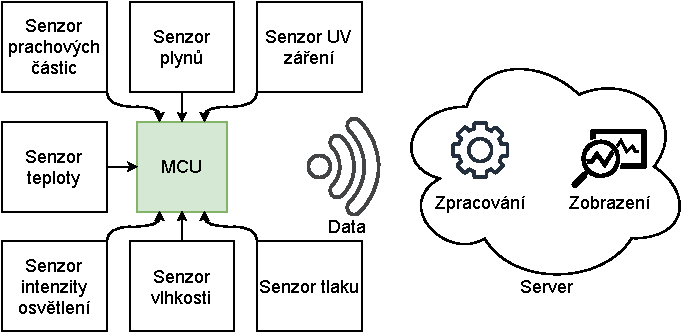
\includegraphics{obrazky/block_schematic-blank.drawio.pdf}
    \caption{Blokový diagram výsledné funkce zařízení.}
    \label{fig_BlockDiagram-blank}
\end{figure}

%%% Vložení souboru 'text/cile.tex' s úvodem
\chapter*{Cíle práce}
\phantomsection
\addcontentsline{toc}{chapter}{Cíle práce}

Konkrétní specifikace cílů, které má autor v~práci vyřešit.
Tato kapitola je \emph{volitelná} -- pokud váš studijní program nevyžaduje zvláštní kapitolu s~cíli,
cíle specifikujte v~rámci Úvodu.

%%% Vložení souboru 'text/reseni' s popisem řešení práce
% (rozdělte na více souborů či kapitol, pokud je vhodné)
\chapter{Návrh zařízení}

Tato kapitola se bude zabývat návrhem hardwaru celého zařízení. Jedním z hlavních požadavků je nízká spotřeba, kterou bude třeba zohlednit při vybírání použitých senzorů, řídícího mikroprocesoru, komunikačního modulu a ostatních obvodových komponent. 

\section{Výběr senzorů}
Celé zařízení bude schopno měřit koncentraci prachových částic, koncentraci oxidu uhelnatého, intenzitu osvětlení, intenzitu UV záření, teplotu, atmosférický tlak a relativní vlhkost. V následujících částech tedy bude popsán výběr z dostupných senzorů.

\subsection{Senzor koncentrace prachových částic}

Na trhu je dostupných hned několik senzorů na měření koncentrace prachových částic. Jak již bylo zmíněno v teoretickém úvodu, budu vybírat senzor, který tuto koncentraci určuje na základě osvícení daného vzorku vzduchu a následně měření odraženého světla. Nyní vyvstává otázka, jestli zvolit senzor, který bude vzorek vzduchu vhánět do měřícího prostoru nuceně pomocí ventilátoru nebo jen za využití stoupání teplého vzduchu nahoru. V tabulce \ref{tab_DustSensors} jsou uvedeny senzory, které jsou relativně cenově přijatelné, a~daly by se pro neprofesionální měření využít.

\newcommand{\ugcm}{\micro\gram\per\cubic\meter} % define new command used in '\SI' -> micro gram per cubic meter

\begin{table}[h]
    \centering
    \begin{tabular}{c|cccc}
    \textbf{Název}           & \textbf{Rozlišení}                & \textbf{Přesnost}                              & \textbf{Proud}                           & \textbf{Čas čtení}                \\ \hline
    \multirow{2}{*}{PMS5003} & \multirow{2}{*}{\SI{1}{\ugcm}}    & $0-100$\SI{}{\ugcm}:$\pm$\SI{10}{\micro\gram}  & \multirow{2}{*}{\SI{100}{\milli\ampere}} & \multirow{2}{*}{\SI{10}{\second}} \\
                             &                                   & $100-500$\SI{}{\ugcm}:$\pm$\SI{10}{\percent}   &                                          &                                   \\ \hline
    \multirow{2}{*}{PM1003}  & \multirow{2}{*}{\SI{1}{\ugcm}}    & $0-100$\SI{}{\ugcm}:$\pm$\SI{30}{\micro\gram}  & \multirow{2}{*}{\SI{90}{\milli\ampere}}  & \multirow{2}{*}{\SI{30}{\second}} \\
                             &                                   & $100-500$\SI{}{\ugcm}:$\pm$\SI{30}{\percent}   &                                          &                                   \\ \hline
    \multirow{2}{*}{PM1006}  & \multirow{2}{*}{neuvedeno}        & $0-100$\SI{}{\ugcm}:$\pm$\SI{20}{\micro\gram}  & \multirow{2}{*}{\SI{30}{\milli\ampere}}  & \multirow{2}{*}{\SI{8}{\second}}  \\
                             &                                   & $100-500$\SI{}{\ugcm}:$\pm$\SI{20}{\percent}   &                                          &                                   \\ \hline
    GP2Y1010AU0F             & \SI{0,5}{\volt}$/$\SI{100}{\ugcm} & záleží na ADC                                  & \SI{20}{\milli\ampere}                   & \SI{1}{\second}                           
    \end{tabular}
    \caption{Porovnání vybraných parametrů senzorů koncentrace prachových částic}
    \label{tab_DustSensors}
\end{table}

Po pečlivém prostudování jednotlivých parametrů jsem zvolil senzor PMS5003 od firmy PLANTOWER. Důležitým aspektem při výběru byla také cena tohoto senzoru, v době vypracovávání této práce jej šlo pořídit za zhruba 350~Kč. Dalším důležitým parametrem byla spotřeba proudu v aktivním stavu, na první pohled se může zdát, že oproti všem senzorům má spotřebu nejvyšší. Oproti PM1003 má však třetinový čas potřebný k získání měřených dat, takže spotřebovává sice vyšší proud, ale po kratší časový úsek. PM1006 má spotřebu proudu zhruba třetinovou, ale vzorek měřeného vzduchu se do měřícího prostoru dostává pomocí sálání a tak je nutné zajistit konstrukčně dostatečně a správně dimenzované průduchy a také konstantní polohu a hlavně náklon senzoru, což by mohlo být v praxi téměř nemožné, pokud má být zařízení používáno také ve volném prostranství. Poslední ze senzorů v tabulce \ref{tab_DustSensors} má zdánlivě nejlepší výsledky. Bohužel se jedná pouze o měřící modul samotný, který neobsahuje žádný ventilátor ani řídící logiku, je tedy třeba tyto věci zapojit a konstrukčně vyřešit. Nejjednodušší na obvodové zapojení, a i z hlediska parametrů přesnosti nejlepší, se tak jeví již zmíněný senzor PMS5003. Senzor potřebuje pro svou funkci napájení \SI{5}{\volt}, a~komunikuje přes rozhraní UART.

\begin{figure}
    \centering
    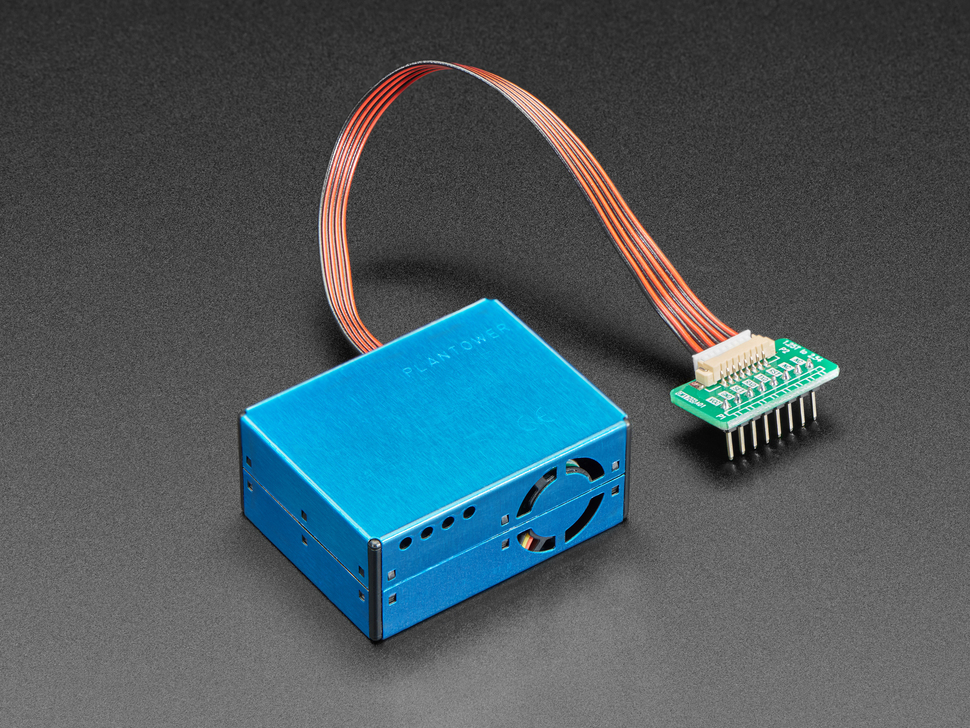
\includegraphics[width=0.7\textwidth]{obrazky/PMS5003.jpg}
    \caption{Senzor pro měření koncentrace prachových částic PMS5003. \cite{dat_PMS5003}}
    \label{fig_PMS5003}
\end{figure}

\subsection{Senzor oxidu uhelnatého}

U senzorů oxidu uhelnatého je situace o něco složitější. Na trhu neexistuje mnoho možností, ze kterých by se dalo v rozumné cenové kategorii vybírat. Pokud se podíváme do katalogů většiny (nejen českých) obchodů, zjistíme, že ceny čidel se pohybují ve vyšších stovkách korun až po několik tisíc. Tato cena je pro neprofesionální měření nepřijatelná. Jediným možným rozumným výběrem jsou čidla s označením série MQ od výrobce Hanwei electronics\footnote{\url{https://www.hwsensor.com/}}. Vybral jsem tedy čidlo s označením MQ-7, které je nejvíce citlivé právě na oxid uhelnatý. Funguje na principu ohřevu senzitivní vrstvy (zde konkrétně z materiálu $SnO_{2}$) a následně měření jejího odporu. Senzor je třeba napájet z \SI{5}{\volt} a jeho výstup je třeba přivést na AD převodník, jelikož má analogový výstup.

\begin{figure}
    \centering
    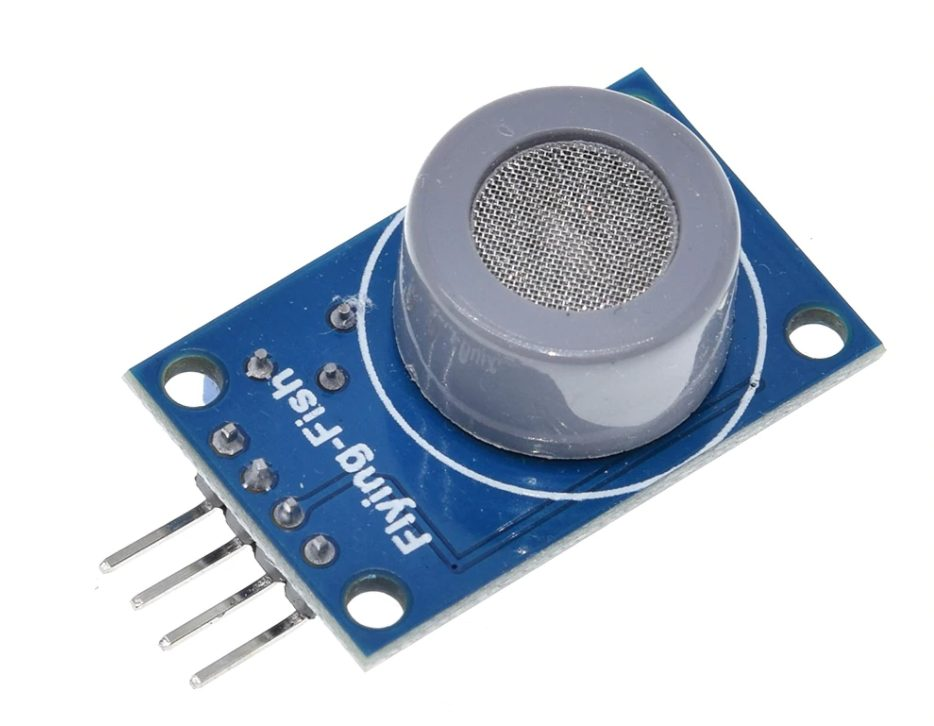
\includegraphics[width=0.7\textwidth]{obrazky/mq7.jpg}
    \caption{Senzor pro měření koncentrace oxidu uhelnatého. \cite{img_mq7}}
    \label{fig_MQ7}
\end{figure}

\subsection{Senzor UV záření}

Na poli relativně levných UV senzorů je výběr opět o něco horší. Existují v podstatě dvě varianty použitelné pro neprofesionální měření a to senzor VEML6075 od výrobce VISHAY a senzor ML8511 výrobce LAPIS Semiconductor. Bohužel první ze zmíněných senzorů se nedá rozumně sehnat, skladové zásoby jsou vyprodané a několik obchodů udává, že se již nevyrábí.

Volím tedy druhý zmíněný senzor ML8511. Tento senzor měří pouze intenzitu UV záření pomocí fotodiody, která je citlivá na UVA a UVB záření. Její největší citlivost je dle datasheetu \cite{dat_ML8511} na vlnovou délku \SI{365}{\nano\metre}. Pro svou činnost potřebuje napájení \SI{3,3}{\volt} a během měření je jeho maximální spotřeba \SI{500}{\micro\ampere}. Pokud jej uvedeme pomocí pinu EN do režimu standby, tak může být spotřeba maximálně \SI{1}{\micro\ampere}. Výstup senzoru je opět napěťový, takže musíme jeho výstup přivést na AD převodník. Rozsah těchto napětí je zhruba od \SI{1}{\volt} do \SI{3}{\volt}, což odpovídá rozsahu \SI{0}{} až \SI{15}{\milli\watt\per\centi\metre\squared}

\subsection{Senzor teploty}

Na poli senzorů pro měření teploty existuje nepřeberné množství různých druhů od spousty výrobců. Pro první základní výběr vhodných senzorů je nutné si definovat alespoň základní parametry a požadavky na takovýto senzor. Vhodnými parametry jsou cena, rozsah měřených teplot (je třeba měřit i při teplotách nižších než \SI{0}{\celsius}), spotřeba a přesnost. Srovnání potenciálně použitelných senzorů se nachází v tabulce \ref{tab_TemperatureSensors}. Cena uvedená v posledním sloupci je brána v jeden den z jednoho e-shopu\footnote{\url{https://www.laskarduino.cz/}}, aby bylo možné objektivně porovnat výsledky mezi sebou.

\begin{table}[]
    \centering
    \begin{tabular}{c|cccc}
    \textbf{Název} & \textbf{Rozsah}                         & \textbf{Přesnost}       & \textbf{Spotřeba}       & \textbf{Cena} \\ \hline
    DS18B20        & \SI{-55}{\celsius} - \SI{125}{\celsius} & $\pm$\SI{0,5}{\celsius} & \SI{1,5}{\milli\ampere} & 68~Kč         \\
    LM75A          & \SI{-25}{\celsius} - \SI{100}{\celsius} & $\pm$\SI{2}{\celsius}   & \SI{280}{\micro\ampere} & 25~Kč         \\
    SHT31          & \SI{-40}{\celsius} - \SI{90}{\celsius}  & $\pm$\SI{0,3}{\celsius} & \SI{350}{\micro\ampere} & 158~Kč        \\
    SHT35          & \SI{-40}{\celsius} - \SI{90}{\celsius}  & $\pm$\SI{0,2}{\celsius} & \SI{1,5}{\milli\ampere} & 378~Kč        \\
    SHT40          & \SI{-40}{\celsius} - \SI{125}{\celsius} & $\pm$\SI{0,2}{\celsius} & \SI{350}{\micro\ampere} & 109~Kč             
    \end{tabular}
    \caption{Srovnání parametrů vybraných senzorů teploty.}
    \label{tab_TemperatureSensors}
\end{table}

Z tabulky \ref{tab_TemperatureSensors} jsem nakonec pro svou práci vybral senzor SHT40 od výrobce SENSIRION. Bohužel není úplně nejlevnější, ale vybral jsem jej díky jeho nízké spotřebě \SI{350}{\micro\ampere} při měření a až \SI{3,4}{\micro\ampere} v nečinném stavu a také relativně vysoké přesnosti, která je až \SI{0,2}{\celsius}. Napájení senzoru je \SI{3,3}{\volt}. S mikroprocesorem senzor komunikuje pomocí sběrnice I$^2$C. 

\begin{figure}
    \centering
    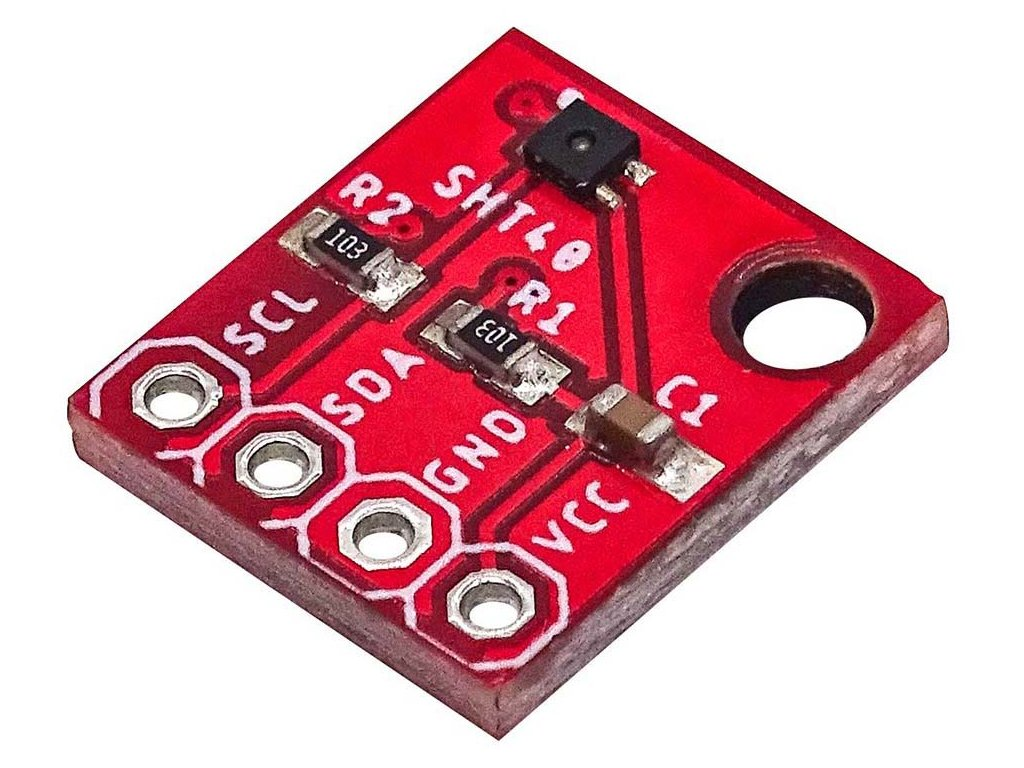
\includegraphics[width=0.55\textwidth]{obrazky/sht40.jpg}
    \caption{Senzor pro měření teploty SHT40. \cite{SHT40}}
    \label{fig_SHT40}
\end{figure}

\subsection{Senzor intenzity osvětlení}

Na poli senzorů pro měření intenzity osvětlení existuje hned několik dostupných variant. Liší se převážně způsobem, jakým intenzitu měří a pak také rozsahem, pro které je možné jejich použití. Pro orientační měření lze využít i prostého fotorezistoru, který zapojíme společně s odporem do série a vytvoříme si tak napěťový dělič, na kterém budeme měřiti pomocí AD převodníku analogové napětí. Tento typ měření je však silně závislý na použitém typu fotorezistoru a většinou nebývá moc přesné. Využití této metody je spíše pro účely orientačního měření a určení základních informací a to, jestli je tma či jestli je světlo. 

Dalším z možných typů senzorů je využití fototranzistoru nebo fotodiody. Toto měření je přesnější než předchozí zmíněná metoda, ale vyžaduje znalost přechodové charakteristiky součástky a pro přesnější měření i kalibraci vůči známé referenční hodnotě intenzity osvětlení.

Mnohem vhodnějším typem senzorů pro toto konkrétní použití je tak integrovaný senzor, který obsahuje jednak samotnou na světlo citlivou vrstvu a druhak i řídící logiku, která nám poskytuje digitální výstup ze senzoru například ve formě sériové sběrnice.

V tabulce \ref{tab_LuxIntensitySensors} jsou uvedeny vybrané druhy integrovaných senzorů a jejich základní vlastnosti.

\begin{table}[h]
    \centering
    \begin{tabular}{c|cc}
        \textbf{Název} & \textbf{Rozsah}            & \textbf{Spotřeba}         \\ \hline
        GY-302 BH1750  & \SI{0}{}-\SI{65535}{\lux}  & \SI{200}{\micro\ampere}   \\
        TSL2561        & \SI{0}{}-\SI{40000}{\lux}  & \SI{0,6}{\milli\ampere}   \\
        VEML7700       & \SI{0}{}-\SI{120000}{\lux} & \SI{50}{\micro\ampere}
    \end{tabular}
    \caption{Srovnání parametrů vybraných senzorů intenzity osvětlení.}
    \label{tab_LuxIntensitySensors}
\end{table}

Z těchto vybraných dostupných senzorů jsem zvolil poslední z tabulky VEML7700. Tento senzor má velmi nízkou spotřebu i při nejrychlejším cyklu čtení (\SI{100}{\milli\second}) a největší rozsah možného měření. Při porovnání cen se nachází zhruba ve stejné cenové hladině jako druhý nejlepší z této tabulky GY-302~BH1750. S mikrokontrolerem senzor bude komunikovat pomocí sběrnice I$^2$C a napájen bude z \SI{3,3}{\volt}.

\begin{figure}[h!]
    \centering
    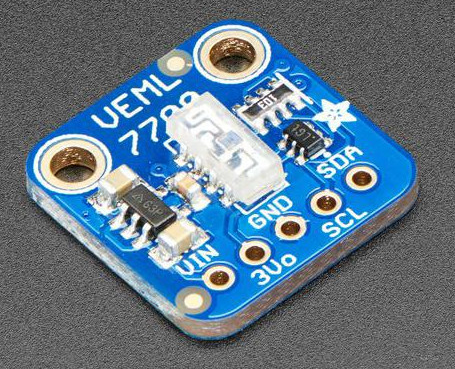
\includegraphics[width=0.4\textwidth]{obrazky/veml7700.png}
    \caption{Senzor pro měření intenzity osvětlení VEML7700. \cite{VEML7700}}
    \label{fig_VEML7700}
\end{figure}

\subsection{Senzor atmosférického tlaku}

Posledním z potřebných senzorů je senzor pro měření atmosférického tlaku. Existuje několik senzorů, které integrují do jednoho pouzdra měření teploty, vlhkosti i atmosférického tlaku. Tyto senzory se však vyznačují nižší přesností. Jedním z takovýchto senzorů je například BME280 od výrobce Bosch, který je populární mezi kutily při stavění amatérské domácí meteostanice. Bohužel poslední dobou není dostupný skladem v žádném z velkých obchodů a pokud se někde vyskytne, stojí několikanásobek jeho normální ceny a je tak pro tuto práci nepoužitelný.

Budu tedy porovnávat senzory, které měří pouze atmosférický tlak a jsou dostupné a mají relativně nízkou cenu.

\begin{table}
    \centering
    \begin{tabular}{c|ccc}
        \textbf{Název} & \textbf{Rozsah}                     & \textbf{Přesnost}      & \textbf{Spotřeba}        \\ \hline
        BMP180         & \SI{300}{}-\SI{1100}{\hecto\pascal} & $\pm$\SI{3}{\pascal}   & \SI{12}{\micro\ampere}   \\
        BMP280         & \SI{300}{}-\SI{1100}{\hecto\pascal} & $\pm$\SI{1,3}{\pascal} & \SI{2,7}{\micro\ampere}  \\
        BMP388         & \SI{300}{}-\SI{1250}{\hecto\pascal} & $\pm$\SI{8}{\pascal}   & \SI{3,4}{\micro\ampere}  \\
        BME280         & \SI{300}{}-\SI{1100}{\hecto\pascal} & $\pm$\SI{2}{\pascal}   & \SI{7,1}{\micro\ampere}  \\
        ICP-10100      & \SI{300}{}-\SI{1150}{\hecto\pascal} & $\pm$\SI{3,2}{\pascal} & \SI{10,4}{\micro\ampere} 
    \end{tabular}
    \caption{Srovnání parametrů vybraných senzorů atmosférického tlaku.}
    \label{tab_AirPressureSensors}
\end{table}

Jak je uvedeno v tabulce \ref{tab_AirPressureSensors}, je vidět že většina senzorů atmosférického tlaku je od výrobce Bosch Sensortec. Vyskytuje se zde již zmiňovaný BME280, který je ale moc drahý a momentálně nedostupný a při měření tlaku má jednu z vyšších spotřeb. Dalším ideálním adeptem by byl i senzor BMP280, který umožňuje měřit atmosférický tlak i teplotu. Bohužel ani tento senzor není příliš dostupný a dle oficiálních stránek výrobce již není doporučen pro nové návrhy.

Vybral jsem tedy senzor BMP388 od firmy Bosch Sensortec. Nepatří bohužel mezi nejlevnější, ale zato je dostupný v obchodech a poskytuje vzhledem ke své dostupnosti relativně dobré parametry samotného měření. Stejně jako dříve zmíněné senzory, i tento senzor umožňuje kromě atmosférického tlaku měřit i teplotu. Pro komunikaci s mikrokontrolerem lze použít sběrnici I$^2$C nebo SPI, jelikož je většina vybraných senzorů na sběrnici I$^2$C, použiji stejnou sběrnici i pro tento senzor. Napájení je třeba přivést \SI{3,3}{\volt}.

\subsection{Senzor měření vlhkosti}

Jak již bylo zmíněno v kapitole o výběru senzoru pro měření teploty, vybraný senzor SHT40 umožňuje měřit i vzdušnou vlhkost. Rozsah měření je \SI{0}{}-\SI{100}{\percent} relativní vlhkosti s přeností $\pm$\SI{1,8}{\percent}. Pro potřeby měření vzdušné vlhkosti v této práci jsou tyto parametry s přehledem dostatečné.

%%% Vložení souboru 'text/vysledky' s popisem vysledků práce
% (rozdělte na více souborů či kapitol, pokud je vhodné)
\chapter{Výsledky studentské práce}

Praktická část a výsledky studentské práce vhodně rozdělené do částí.

\section{Programové řešení}
Lorem ipsum dolor sit amet, consectetuer adipiscing elit. Nulla pulvinar eleifend sem. Integer in sapien. Etiam sapien elit, consequat eget, tristique non, venenatis quis, ante. In laoreet, magna id viverra tincidunt, sem odio bibendum justo, vel imperdiet sapien wisi sed libero. Phasellus enim erat, vestibulum vel, aliquam a, posuere eu, velit. Aliquam erat volutpat. Nullam faucibus mi quis velit \cite{sr02/2009}.

\section{Výsledky měření}
Fusce tellus odio, dapibus id fermentum quis, suscipit id erat. Fusce tellus. Morbi scelerisque luctus velit. In laoreet, magna id viverra tincidunt, sem odio bibendum justo, vel imperdiet sapien wisi sed libero. Quisque porta. Fusce suscipit libero eget elit. Nulla non lectus sed nisl molestie malesuada. Phasellus faucibus molestie nisl. Integer vulputate sem a nibh rutrum consequat. Proin mattis lacinia justo. Phasellus et lorem id felis nonummy placerat. Etiam ligula pede, sagittis quis, interdum ultricies, scelerisque eu. Cras elementum. Aenean placerat. Donec ipsum massa, ullamcorper in, auctor et, scelerisque sed, est. Aliquam ante. Integer imperdiet lectus quis justo. Vivamus ac leo pretium faucibus. Nullam faucibus mi quis velit.

\subsection{Etiam quis quam}
Neque porro quisquam est, qui dolorem ipsum quia dolor sit amet, consectetur, adipisci velit, sed quia non numquam eius modi tempora incidunt ut labore et dolore magnam aliquam quaerat voluptatem. Aliquam erat volutpat. Lorem ipsum dolor sit amet, consectetuer adipiscing elit \cite{sr02/2009,pravidla}. Nunc auctor. Neque porro quisquam est, qui dolorem ipsum quia dolor sit amet, consectetur, adipisci velit, sed quia non numquam eius modi tempora incidunt ut labore et dolore magnam aliquam quaerat voluptatem. Maecenas lorem. Maecenas libero. In laoreet, magna id viverra tincidunt, sem odio bibendum justo, vel imperdiet sapien wisi sed libero. Nullam rhoncus aliquam metus.

\subsubsection{Integer rutrum orci vestibulum}
Integer rutrum, orci vestibulum ullamcorper ultricies, lacus quam ultricies odio, vitae placerat pede sem sit amet enim. Ut enim ad minim veniam, quis nostrud exercitation ullamco laboris nisi ut aliquip ex ea commodo consequat. Fusce tellus odio, dapibus id fermentum quis, suscipit id erat. Nullam eget nisl. Nunc auctor. Etiam dui sem, fermentum vitae, sagittis id, malesuada in, quam. Fusce dui leo, imperdiet in, aliquam sit amet, feugiat eu, orci. Curabitur vitae diam non enim vestibulum interdum. Aliquam erat volutpat. Pellentesque sapien. Phasellus enim erat, vestibulum vel, aliquam a, posuere eu, velit.

\subsubsection{Eger rutrum orci westibulum}
Fusce dui leo, imperdiet in, aliquam sit amet, feugiat eu, orci. Maecenas aliquet accumsan leo. Aliquam ornare wisi eu metus. Cum sociis natoque penatibus et magnis dis parturient montes, nascetur ridiculus mus. Aliquam erat volutpat. Donec iaculis gravida nulla. Sed elit dui, pellentesque a, faucibus vel, interdum nec, diam. Temporibus autem quibusdam et aut officiis debitis aut rerum necessitatibus saepe eveniet ut et voluptates repudiandae sint et molestiae non recusandae. Nulla non arcu lacinia neque faucibus fringilla. Phasellus enim erat, vestibulum vel, aliquam a, posuere eu, velit. Praesent vitae arcu tempor neque lacinia pretium
\cite{Walter1999,Svacina1999IEEE,RajmicSysel2002}.

Aliquam erat volutpat. Quisque porta. Integer imperdiet lectus quis justo. Nullam justo enim, consectetuer nec, ullamcorper ac, vestibulum in, elit. Nullam faucibus mi quis velit. Fusce tellus. Fusce consectetuer risus a nunc. Cras pede libero, dapibus nec, pretium sit amet, tempor quis. Morbi imperdiet, mauris ac auctor dictum, nisl ligula egestas nulla, et sollicitudin sem purus in lacus
\cite{CSN_ISO_690-2011,CSN_ISO_7144-1997,CSN_ISO_31-11}.
Mauris elementum mauris vitae tortor. Neque porro quisquam est, qui dolorem ipsum quia dolor sit amet, consectetur, adipisci velit, sed quia non numquam eius modi tempora incidunt ut labore et dolore magnam aliquam quaerat voluptatem. Quisque porta. Integer vulputate sem a nibh rutrum consequat. Nulla pulvinar eleifend sem. Praesent id justo in neque elementum ultrices \cite{BiernatovaSkupa2011:CSNISO690komentar}.

Fusce suscipit libero eget elit. Integer vulputate sem a nibh rutrum consequat. Aliquam erat volutpat. Etiam neque. Nulla turpis magna, cursus sit amet, suscipit a, interdum id, felis. Nullam rhoncus aliquam metus. Etiam dui sem, fermentum vitae, sagittis id, malesuada in, quam. Nunc auctor. Nunc dapibus tortor vel mi dapibus sollicitudin. Praesent in mauris eu tortor porttitor accumsan. Nulla non arcu lacinia neque faucibus fringilla. Nullam lectus justo, vulputate eget mollis sed, tempor sed magna. Maecenas lorem. Aenean placerat. Donec vitae arcu. Maecenas lorem. Donec iaculis gravida nulla. Nulla non lectus sed nisl molestie malesuada.

Duis pulvinar. Nulla est. Duis condimentum augue id magna semper rutrum. Integer pellentesque quam vel velit. Aliquam ante. Nulla quis diam. Proin mattis lacinia justo. Aenean fermentum risus id tortor. Nunc auctor. Nullam justo enim, consectetuer nec, ullamcorper ac, vestibulum in, elit. In dapibus augue non sapien. Etiam bibendum elit eget erat. In sem justo, commodo ut, suscipit at, pharetra vitae, orci. Maecenas libero.

Nulla non lectus sed nisl molestie malesuada. Donec vitae arcu. Aenean fermentum risus id tortor. Praesent in mauris eu tortor porttitor accumsan. Nulla pulvinar eleifend sem. Duis viverra diam non justo. Integer imperdiet lectus quis justo. Pellentesque habitant morbi tristique senectus et netus et malesuada fames ac turpis egestas. In rutrum. Excepteur sint occaecat cupidatat non proident, sunt in culpa qui officia deserunt mollit anim id est laborum. Nulla non lectus sed nisl molestie malesuada. Aliquam erat volutpat. Mauris tincidunt sem sed arcu. Duis bibendum, lectus ut viverra rhoncus, dolor nunc faucibus libero, eget facilisis enim ipsum id lacus. Fusce tellus odio, dapibus id fermentum quis, suscipit id erat. In enim a arcu imperdiet malesuada. Nulla non lectus sed nisl molestie malesuada. Proin mattis lacinia justo.

Aliquam in lorem sit amet leo accumsan lacinia. Cum sociis natoque penatibus et magnis dis parturient montes, nascetur ridiculus mus. Duis sapien nunc, commodo et, interdum suscipit, sollicitudin et, dolor. Suspendisse sagittis ultrices augue. Nullam lectus justo, vulputate eget mollis sed, tempor sed magna. In convallis. Praesent id justo in neque elementum ultrices. Neque porro quisquam est, qui dolorem ipsum quia dolor sit amet, consectetur, adipisci velit, sed quia non numquam eius modi tempora incidunt ut labore et dolore magnam aliquam quaerat voluptatem.

Pellentesque pretium lectus id turpis. Nemo enim ipsam voluptatem quia voluptas sit aspernatur aut odit aut fugit, sed quia consequuntur magni dolores eos qui ratione voluptatem sequi nesciunt. Curabitur ligula sapien, pulvinar a vestibulum quis, facilisis vel sapien. Praesent dapibus. Sed elit dui, pellentesque a, faucibus vel, interdum nec, diam. Duis viverra diam non justo. Duis ante orci, molestie vitae vehicula venenatis, tincidunt ac pede. Phasellus rhoncus. Maecenas fermentum, sem in pharetra pellentesque, velit turpis volutpat ante, in pharetra metus odio a lectus. Proin pede metus, vulputate nec, fermentum fringilla, vehicula vitae, justo. Fusce aliquam vestibulum ipsum. Nullam at arcu a est sollicitudin euismod.

%Aliquam ante. Phasellus faucibus molestie nisl. Etiam ligula pede, sagittis quis, interdum ultricies, scelerisque eu. Morbi leo mi, nonummy eget tristique non, rhoncus non leo. Cum sociis natoque penatibus et magnis dis parturient montes, nascetur ridiculus mus. Morbi scelerisque luctus velit. Curabitur bibendum justo non orci. Donec quis nibh at felis congue commodo. Nullam faucibus mi quis velit. Aenean id metus id velit ullamcorper pulvinar. Pellentesque sapien. Fusce nibh. Vestibulum fermentum tortor id mi. Nullam eget nisl. Praesent vitae arcu tempor neque lacinia pretium. Proin in tellus sit amet nibh dignissim sagittis. Donec quis nibh at felis congue commodo.
%
%Nam quis nulla. Proin in tellus sit amet nibh dignissim sagittis. Nullam dapibus fermentum ipsum. Curabitur ligula sapien, pulvinar a vestibulum quis, facilisis vel sapien. Nam libero tempore, cum soluta nobis est eligendi optio cumque nihil impedit quo minus id quod maxime placeat facere possimus, omnis voluptas assumenda est, omnis dolor repellendus. Vivamus ac leo pretium faucibus. Nunc tincidunt ante vitae massa. Maecenas sollicitudin. Ut tempus purus at lorem. Nullam lectus justo, vulputate eget mollis sed, tempor sed magna. Fusce consectetuer risus a nunc. Etiam quis quam.
%
%Donec quis nibh at felis congue commodo. Sed vel lectus. Donec odio tempus molestie, porttitor ut, iaculis quis, sem. Nullam feugiat, turpis at pulvinar vulputate, erat libero tristique tellus, nec bibendum odio risus sit amet ante. Sed elit dui, pellentesque a, faucibus vel, interdum nec, diam. Cras elementum. Sed vel lectus. Donec odio tempus molestie, porttitor ut, iaculis quis, sem. Etiam neque. Integer tempor. Vivamus porttitor turpis ac leo. Nulla non arcu lacinia neque faucibus fringilla.
%
%Etiam posuere lacus quis dolor. Nemo enim ipsam voluptatem quia voluptas sit aspernatur aut odit aut fugit, sed quia consequuntur magni dolores eos qui ratione voluptatem sequi nesciunt. Nullam faucibus mi quis velit. Cum sociis natoque penatibus et magnis dis parturient montes, nascetur ridiculus mus. Phasellus faucibus molestie nisl. Maecenas ipsum velit, consectetuer eu lobortis ut, dictum at dui. Maecenas aliquet accumsan leo. Pellentesque ipsum. Donec vitae arcu. Suspendisse nisl. Morbi imperdiet, mauris ac auctor dictum, nisl ligula egestas nulla, et sollicitudin sem purus in lacus. Pellentesque ipsum. Ut enim ad minima veniam, quis nostrum exercitationem ullam corporis suscipit laboriosam, nisi ut aliquid ex ea commodi consequatur? Nam libero tempore, cum soluta nobis est eligendi optio cumque nihil impedit quo minus id quod maxime placeat facere possimus, omnis voluptas assumenda est, omnis dolor repellendus.


%%% Vložení souboru 'text/zaver' se závěrem
\chapter*{Závěr}
\phantomsection
\addcontentsline{toc}{chapter}{Závěr}

V teoretickém úvodu byly rozebrány jednotlivé technologie senzorů pro měření daných veličin a~možnosti přenášení naměřených dat na server. Následně byly vybrány všechny potřebné senzory s~ohledem na kvalitativní parametry a~co nejnižší provozní spotřebu pro dosažení co nejdelšího provozu při provozu z~baterie. Jako síť pro přenos dat byly vybrány dvě možnosti. První je LoRaWAN ve spojení s komunitním serverem The Things Network, tato síť umožňuje připojení zařízení a odesílání dat kdekoliv, kde se vyskytuje gateway zapojená do tohoto projektu. Druhou sítí, použitelnou například v domácích podmínkách, je WiFi. Nedílnou součástí výběru hardwarových komponent byl výběr řídícího mikrokontroleru, kde bylo zapotřebí vybrat vhodný typ podle potřebných komunikačních sběrnic a~hardwarových prostředků. Nakonec byl vybrán mikrokontroler ESP32, jelikož má všechny potřebné periferie a~umožňuje dosáhnout při různých provozních režimech velice nízké spotřeby.

Po sestavení výsledného blokového schématu byly navrženy obvodové zapojení a také desky plošných spojů v programu KiCad. Kromě hlavní řídící desky, která má rozměry $50 \times 50$\SI{}{\milli\metre} a obsahuje většinu senzorů a veškerou řídící elektroniku. Tuto hlavní desku doplňuje menší deska s dvěma senzory pro měření parametrů osvětlení a je nasazena na tuto hlavní desku. Celé zařízení bylo navrhováno s ohledem na co nejnižší spotřebu a tudíž i provoz na baterie. Z tohoto důvodu jsou vypínatelné veškeré senzory a komunikační moduly tak, aby v režimu hlubokého spánku byl v provozu pouze časovač v mikrokontroleru, který zařízení po definovaném čase opět probudí. Díky tomuto návrhu se podařilo vyrobit zařízení, které má v režimu hlubokého spánku spotřebu pouhých \SI{5.8}{\micro\ampere}. Při napájení baterií LiFePO4 s kapacitou \SI{3200}{\milli\ampere\hour} a periodou měření a odesílání dat \SI{1}{\hour} je teoreticky možné dosáhnout výdrže až 160~dní.

Pro možnost nabíjení baterie přímo v zařízení bez nutnosti jej rozebírat byla dále navržena nabíjecí deska. Tato nabíječka umožňuje připojení k hlavní desce i v průběhu její činnosti. Nabíječku lze napájet napětím \SI{5}{} až \SI{40}{\volt}. Na její vstup může být připojen solární panel a aktivována integrovaná MPPT funkce obvodu. S tímto zapojením je tak možné i s velice malým solárním panelem dosáhnout nepřetržité funkce zařízení.

Po sestavení a oživení zařízení bylo zapotřebí naprogramovat potřebné funkce. Firmware je založen na frameworku ESP-IDF od samotného výrobce čipu Espressif. Byly napsány veškeré obslužné knihovny pro senzory a zajištěna možnost uživatelského výběru a konfigurace připojení k síti LoRaWAN či WiFi. Při psaní firmwaru bylo také dbáno na optimalizaci spotřeby zařízení a zejména co nejkratší běh samotného měření a odesílání. Proto jsou využity vícevláknové operace a celý cyklus od probuzení mikrokontroleru přes měření až po odeslání dat trvá v průměru \SI{30}{\second}.

Důležitým rozhodnutím pro celou práci bylo, jakým způsobem uživateli předat v grafické podobě naměřená data. V práci byly rozebrány různé možnosti veřejně dostupných serverů. Nakonec bylo vybráno vlastní řešení poskládané z konkrétních služeb a aplikací, které jsem nainstaloval na Raspberry Pi 4. Toto vlastní řešení má výhodu v teoreticky neomezeném množství přenesených dat a připojených zařízení. Pokud by přestalo toto Raspberry Pi výkonostně stačit, stačí tyto služby pouze nainstalovat například na pronajatý server a lze celé řešení výkonnostně škálovat. Nevýhodou tohoto Rapsberry Pi je, že pokud vypadne elektřina nebo internet, tak se posílaná data ztratí a nebudou přijaty. Tento neduh může opět odstranit hostování v cloudu.

Poslední prací bylo navrhnutí a vytištění krabičky na 3D tiskárně pro veškerou elektroniku a senzory. Poté bylo sestaveno celé zařízení a zprovozněno. Celkové náklady na sestavení se v květnu 2022 pohybovaly okolo $1630$~Kč. V ceně není zahrnuta nabíječka ani 3D tisk krabičky.

%%% Vložení souboru 'text/literatura' se seznamem zdrojů
% Pro sazbu seznamu literatury použijte jednu z následujících možností

%%%%%%%%%%%%%%%%%%%%%%%%%%%%%%%%%%%%%%%%%%%%%%%%%%%%%%%%%%%%%%%%%%%%%%%%%
%1) Seznam citací definovaný přímo pomocí prostředí literatura / thebibliography

\begin{thebibliography}{99}
	
\bibitem{sr02/2009}
		VUT v~Brně:
    \emph{Úprava, odevzdávání a zveřejňování vysokoškolských kva\-li\-fi\-kač\-ních prací na VUT v~Brně}\/ [online].
		Směrnice rektora č.\,2/2009.
		Brno: 2009, po\-sled\-ní aktualizace 24.\,3.\,2009 [cit.\,23.\,10.\,2015].
    Dostupné z~URL:\\
    <\url{https://www.vutbr.cz/uredni-deska/vnitrni-predpisy-a-dokumenty/smernice-rektora-f34920/}>.

\bibitem{CSN_ISO_690-2011}
    \emph{ČSN ISO 690 (01 0197) Informace a dokumentace -- Pravidla pro bibliografické odkazy a citace informačních zdrojů.}
    40 stran. Praha: Český normalizační institut, 2011.

\bibitem{CSN_ISO_7144-1997}
    \emph{ČSN ISO 7144 (010161) Dokumentace -- Formální úprava disertací a podobných dokumentů.}
    24 stran. Praha: Český normalizační institut, 1997.

\bibitem{CSN_ISO_31-11}
    \emph{ČSN ISO 31-11 Veličiny a jednotky -- část 11: Matematické znaky a značky používané ve fyzikálních vědách a v~technice.}
    Praha: Český normalizační institut, 1999.

\bibitem{BiernatovaSkupa2011:CSNISO690komentar}
    BIERNÁTOVÁ, O., SKŮPA, J.:
    \emph{Bibliografické odkazy a citace dokumentů dle ČSN ISO 690 (01 0197) platné od 1.\,dubna 2011}\/ [online].
    2011, poslední aktualizace 2.\,9.\,2011 [cit. 19.\,10.\,2011].
    Dostupné z~URL:
    \(<\)\url{http://www.citace.com/CSN-ISO-690.pdf}\(>\)
%    \(<\)\href{http://www.boldis.cz/citace/citace.html}{http://www.boldis.cz/citace/citace.html}\(>\).

\bibitem{pravidla}
    \emph{Pravidla českého pravopisu}.
    Zpracoval kolektiv autorů. 1.\ vydání.
    Olomouc: FIN PUB\-LISH\-ING, 1998. 575 s. ISBN 80-86002-40-3.

\bibitem{Walter1999}
	WALTER, G.\,G.; SHEN, X.
	\emph{Wavelets and Other Orthogonal Systems}.
	2. vyd. Boca Raton: Chapman\,\&\,Hall/CRC, 2000. 392~s. ISBN 1-58488-227-1

\bibitem{Svacina1999IEEE}
	SVAČINA, J.
	Dispersion Characteristics of Multilayered Slotlines -- a Simple Approach.
	\emph{IEEE Transactions on Microwave Theory and Techniques},
	1999, vol.\,47, no.\,9, s.\,1826--1829. ISSN 0018-9480.

\bibitem{RajmicSysel2002}
    RAJMIC, P.; SYSEL, P.
    Wavelet Spectrum Thresholding Rules.
    In \emph{Proceedings of the International Conference Research in Telecommunication Technology},
    Žilina: Žilina University, 2002. s.\,60--63. ISBN 80-7100-991-1.

\end{thebibliography}


% %%%%%%%%%%%%%%%%%%%%%%%%%%%%%%%%%%%%%%%%%%%%%%%%%%%%%%%%%%%%%%%%%%%%%%%%
% %2) Seznam citací pomocí BibTeXu
% % Při použití je nutné v TeXnicCenter ve výstupním profilu aktivovat spouštění BibTeXu po překladu.
% % Definice stylu seznamu
% \bibliographystyle{unsrturl}
% % Pro českou sazbu lze použít styl czechiso.bst ze stránek
% % http://www.fit.vutbr.cz/~martinek/latex/czechiso.tar.gz
% %\bibliographystyle{czechiso}
% % Vložení souboru se seznamem citací
% \bibliography{text/literatura}

% % Následující příkaz je pouze pro ukázku sazby literatury při použití BibTeXu.
% % Způsobí citaci všech zdrojů v souboru literatura.bib, i když nejsou citovány v textu.
% \nocite{*}

%%% Vložení souboru 'text/zkratky' se seznam použitých symbolů, veličin a zkratek
\cleardoublepage
\chapter*{\listofabbrevname}
\phantomsection
\addcontentsline{toc}{chapter}{\listofabbrevname}

\begin{acronym}[KolikMista]

	\acro{zkTemp}		% název
		[Šířka levého sloupce Seznamu symbolů a zkratek]								% zkratka
		{je určena šířkou parametru prostředí \texttt{acronym} (viz řádek~1 výpisu zdrojáku na~str.\,\pageref{lst:zkratky})}
											% rozvinutí zkratky

	\acro{zkDummy}
		[KolikMista]
		{pouze ukázka vyhrazeného místa}

	\acro{DSP}		% název/zkratka
		{číslicové zpracování signálů -- Digital Signal Processing}
											% rozvinutí zkratky
	%%% bsymfvz
	\acro{symfvz}						% název
		[\ensuremath{f_\textind{vz}}] % symbol
		{vzorkovací kmitočet}					% popis
	%%% esymfvz

\end{acronym}


%%% Začátek příloh
\appendix

%%% Vysázení seznamu příloh
% (vynechejte, pokud máte dvě nebo méně příloh)
\listofappendices

%%% Vložení souboru 'text/prilohy' s přílohami
% Obvykle je přítomen alespoň popis co najdeme na přiloženém médiu
% \chapter{Některé příkazy balíčku \texttt{thesis}}

% \section{Příkazy pro sazbu veličin a~jednotek}

% \begin{table}[!h]
%   \caption[Přehled příkazů]{Přehled příkazů pro matematické prostředí }
%   \begin{center}
%   	\small
% 	  \begin{tabular}{|c|c|c|c|}
% 	    \hline
% 	    Příkaz    						& Příklad 					& Zdroj příkladu  							& Význam  \\
% 	    \hline\hline
% 	    \verb|\textind{...}|	& $\beta_\textind{max}$ 	& \verb|$\beta_\textind{max}$|	& textový index \\
% 	    \hline
% 	    \verb|\const{...}| 		& $\const{U}_\textind{in}$ 				& \verb|$\const{U}_\textind{in}$|		& konstantní veličina \\
% 	    \hline
% 	    \verb|\var{...}| 		& $\var{u}_\textind{in}$ & \verb|$\var{u}_\textind{in}$| & proměnná veličina \\
% 	    \hline
% 	    \verb|\complex{...}| 	& $\complex{u}_\textind{in}$ & \verb|$\complex{u}_\textind{in}$| & komplexní veličina \\
% 	    \hline
% 	    \verb|\vect{...}| 		& $\vect{y}$ 						& \verb|$\vect{y}$| & vektor \\
% 	    \hline
% 	    \verb|\mat{...}| 	& $\mat{Z}$ 						& \verb|$\mat{Z}$| & matice \\
% 	    \hline
% 	    \verb|\unit{...}| 		& $\unit{kV}$ 						& \verb|$\unit{kV}$|\quad či\ \, \verb|\unit{kV}| & jednotka \\
% 	    \hline
% 	  \end{tabular}
%   \end{center}
% \end{table}



% %\newpage
% \section{Příkazy pro sazbu symbolů}

% \begin{itemize}
%   \item
%     \verb|\E|, \verb|\eul| -- sazba Eulerova čísla: $\eul$,
%   \item
%     \verb|\J|, \verb|\jmag|, \verb|\I|, \verb|\imag| -- sazba imaginární jednotky: $\jmag$, $\imag$,
%   \item
%     \verb|\dif| -- sazba diferenciálu: $\dif$,
%   \item
%     \verb|\sinc| -- sazba funkce: $\sinc$,
%   \item
%     \verb|\mikro| -- sazba symbolu mikro stojatým písmem%
% 			\footnote{znak pochází z~balíčku \texttt{textcomp}}: $\mikro$,
% 	\item
% 		\verb|\uppi| -- sazba symbolu $\uppi$
% 			(stojaté řecké pí, na rozdíl od \verb|\pi|, což sází $\pi$).
% \end{itemize}
% %
% Všechny symboly jsou určeny pro matematický mód, vyjma \verb|\mikro|, jenž je\\ použitelný rovněž v~textovém módu.
% %$\upmikro$


% \chapter{Druhá příloha}

% \begin{figure}[!h]
%   \begin{center}
%     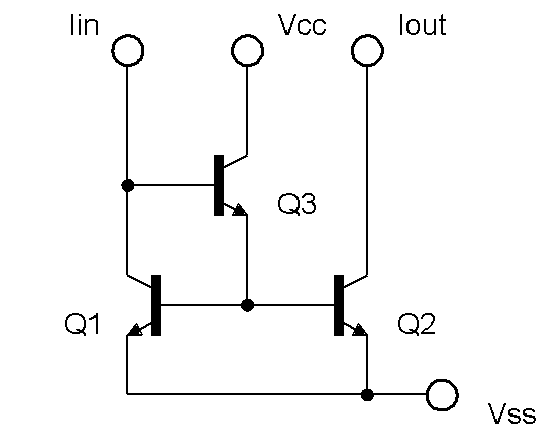
\includegraphics[scale=0.5]{obrazky/ZlepseneWilsonovoZrcadloNPN}
%   \end{center}
%   \caption[Alenčino zrcadlo]{Zlepšené Wilsonovo proudové zrcadlo.}
% \end{figure}

% Pro sazbu vektorových obrázků přímo v~\LaTeX{}u je možné doporučit balíček \href{https://www.ctan.org/pkg/pgf}{\texttt{TikZ}}.
% Příklady sazby je možné najít na \href{http://www.texample.net/tikz/examples/}{\TeX{}ample}.
% Pro vyzkoušení je možné použít programy QTikz nebo TikzEdt.




% \chapter{Příklad sazby zdrojových kódů}

% \section{Balíček \texttt{listings}}

% Pro vysázení zdrojových souborů je možné použít balíček \href{https://www.ctan.org/pkg/listings}{\texttt{listings}}.
% Balíček zavádí nové prostředí \texttt{lstlisting} pro sazbu zdrojových kódů, jako například:
% %
% \begin{lstlisting}[language={[LaTeX]TeX}]
% \section{Balíček lstlistings}
% Pro vysázení zdrojových souborů je možné použít
% 	balíček \href{https://www.ctan.org/pkg/listings}%
% 	{\texttt{listings}}.
% Balíček zavádí nové prostředí \texttt{lstlisting} pro
% 	sazbu zdrojových kódů.
% \end{lstlisting}
% %
% Podporuje množství programovacích jazyků.
% Kód k~vysázení může být načítán přímo ze zdrojových souborů.
% Umožňuje vkládat čísla řádků nebo vypisovat jen vybrané úseky kódu.
% Např.:

% \noindent
% Zkratky jsou sázeny v~prostředí \texttt{acronym}:
% \label{lst:zkratky}
% \lstinputlisting[language={[LaTeX]TeX},nolol,numbers=left, firstnumber=6, firstline=6,lastline=6]{text/zkratky.tex}
% %
% Šířka textu volitelného parametru \verb|KolikMista| udává šířku prvního sloupce se zkratkami.
% Proto by měla být zadávána nejdelší zkratka nebo symbol.
% Příklad definice zkratky \acs{symfvz} je na výpisu \ref{lst:symfvz}.

% \shorthandoff{-}
% \lstinputlisting[language={[LaTeX]TeX},frame=single,caption={Ukázka sazby zkratek},label=lst:symfvz,numbers=left,linerange={bsymfvz-\%\%\%\ esymfvz},includerangemarker=false]{text/zkratky.tex}
% \shorthandon{-}

% \noindent
% Ukončení seznamu je provedeno ukončením prostředí:
% \lstinputlisting[language={[LaTeX]TeX},nolol,numbers=left,firstnumber=26,linerange=26]{text/zkratky.tex}

% \vspace{\fill}

% \noindent
% {\bf Poznámka k~výpisům s~použitím volby jazyka \verb|czech| nebo \verb|slovak|:}\newline
% Pokud Váš zdrojový kód obsahuje znak spojovníku \verb|-|, pak překlad může skončit chybou.
% Ta je způsobená tím, že znak \verb|-| je v~českém nebo slovenském nastavení balíčku \verb|babel| tzv.\ aktivním znakem.
% Přepněte znak \verb|-| na neaktivní příkazem \verb|\shorthandoff{-}| těsně před výpisem a~hned za ním jej vraťte na aktivní příkazem \verb|\shorthandon{-}|.
% Podobně jako to je ukázáno ve zdrojovém kódu šablony.


% \clearpage

% %\section{Výpis kódu prostředí Matlab}
% Na výpisu \ref{lst:priklad.vypis.kodu.Matlab} naleznete příklad kódu pro Matlab, na výpisu \ref{lst:priklad.vypis.kodu.C} zase pro jazyk~C.

% \lstnewenvironment{matlab}[1][]{%
% \iflanguage{czech}{\shorthandoff{-}}{}%
% \iflanguage{slovak}{\shorthandoff{-}}{}%
% \lstset{language=Matlab,numbers=left,#1}%
% }{%
% \iflanguage{slovak}{\shorthandon{-}}{}%
% \iflanguage{czech}{\shorthandon{-}}{}%
% }

% \begin{matlab}[frame=single,float=htbp,caption={Příklad Schur-Cohnova testu stability v~prostředí Matlab.},label=lst:priklad.vypis.kodu.Matlab,numberstyle=\scriptsize, numbersep=7pt]
% %% Priklad testovani stability filtru

% % koeficienty polynomu ve jmenovateli
% a~= [ 5, 11.2, 5.44, -0.384, -2.3552, -1.2288];
% disp( 'Polynom:'); disp(poly2str( a, 'z'))

% disp('Kontrola pomoci korenu polynomu:');
% zx = roots( a);
% if( all( abs( zx) < 1))
%     disp('System je stabilni')
% else
%     disp('System je nestabilni nebo na mezi stability');
% end

% disp(' '); disp('Kontrola pomoci Schur-Cohn:');
% ma = zeros( length(a)-1,length(a));
% ma(1,:) = a/a(1);
% for( k~= 1:length(a)-2)
%     aa = ma(k,1:end-k+1);
%     bb = fliplr( aa);
%     ma(k+1,1:end-k+1) = (aa-aa(end)*bb)/(1-aa(end)^2);
% end

% if( all( abs( diag( ma.'))))
%     disp('System je stabilni')
% else
%     disp('System je nestabilni nebo na mezi stability');
% end
% \end{matlab}

% \noindent
% \begin{minipage}{\linewidth}


% %\section{Výpis kódu jazyka C}

% \begin{lstlisting}[frame=single,numbers=right,caption={Příklad implementace první kanonické formy v~jazyce C.},label=lst:priklad.vypis.kodu.C,basicstyle=\ttfamily\small, keywordstyle=\color{black}\bfseries\underbar,]
% // první kanonická forma
% short fxdf2t( short coef[][5], short sample)
% {
% 	static int v1[SECTIONS] = {0,0},v2[SECTIONS] = {0,0};
% 	int x, y, accu;
% 	short k;

% 	x = sample;
% 	for( k~= 0; k~< SECTIONS; k++){
% 		accu = v1[k] >> 1;
% 		y = _sadd( accu, _smpy( coef[k][0], x));
% 		y = _sshl(y, 1) >> 16;

% 		accu = v2[k] >> 1;
% 		accu = _sadd( accu, _smpy( coef[k][1], x));
% 		accu = _sadd( accu, _smpy( coef[k][2], y));
% 		v1[k] = _sshl( accu, 1);

% 		accu = _smpy( coef[k][3], x);
% 		accu = _sadd( accu, _smpy( coef[k][4], y));
% 		v2[k] = _sshl( accu, 1);

% 		x = y;
% 	}
% 	return( y);
% }
% \end{lstlisting}
% \end{minipage}







% \chapter{Obsah elektronické přílohy}
% Elektronická příloha je často nedílnou součástí semestrální nebo závěrečné práce.
% Vkládá se do informačního systému VUT v~Brně ve vhodném formátu (ZIP, PDF\,\dots).

% Nezapomeňte uvést, co čtenář v~této příloze najde.
% Je vhodné okomentovat obsah každého adresáře, specifikovat, který soubor obsahuje důležitá nastavení, který soubor je určen ke spuštění, uvést nastavení kompilátoru atd.
% Také je dobře napsat, v~jaké verzi software byl kód testován (např.\ Matlab 2018b).
% Pokud bylo cílem práce vytvořit hardwarové zařízení,
% musí elektronická příloha obsahovat veškeré podklady pro výrobu (např.\ soubory s~návrhem DPS v~Eagle).

% Pokud je souborů hodně a~jsou organizovány ve více složkách, je možné pro výpis adresářové struktury použít balíček \href{https://www.ctan.org/pkg/dirtree}{\texttt{dirtree}}.

% \bigskip

% {\small
% %
% \dirtree{%.
% .1 /\DTcomment{kořenový adresář přiloženého archivu}.
% .2 logo\DTcomment{loga školy a~fakulty}.
% .3 BUT\_abbreviation\_color\_PANTONE\_EN.pdf.
% .3 BUT\_color\_PANTONE\_EN.pdf.
% .3 FEEC\_abbreviation\_color\_PANTONE\_EN.pdf.
% .3 FEKT\_zkratka\_barevne\_PANTONE\_CZ.pdf.
% .3 UTKO\_color\_PANTONE\_CZ.pdf.
% .3 UTKO\_color\_PANTONE\_EN.pdf.
% .3 VUT\_barevne\_PANTONE\_CZ.pdf.
% .3 VUT\_symbol\_barevne\_PANTONE\_CZ.pdf.
% .3 VUT\_zkratka\_barevne\_PANTONE\_CZ.pdf.
% .2 obrazky\DTcomment{ostatní obrázky}.
% .3 soucastky.png.
% .3 spoje.png.
% .3 ZlepseneWilsonovoZrcadloNPN.png.
% .3 ZlepseneWilsonovoZrcadloPNP.png.
% .2 pdf\DTcomment{pdf stránky generované informačním systémem}.
% .3 student-desky.pdf.
% .3 student-titulka.pdf.
% .3 student-zadani.pdf.
% .2 text\DTcomment{zdrojové textové soubory}.
% .3 literatura.tex.
% .3 prilohy.tex.
% .3 reseni.tex.
% .3 uvod.tex.
% .3 vysledky.tex.
% .3 zaver.tex.
% .3 zkratky.tex.
% %.2 navod-sablona\_FEKT.pdf\DTcomment{návod na používání šablony}.
% .2 sablona-obhaj.tex\DTcomment{hlavní soubor pro sazbu prezentace k~obhajobě}.
% %.2 readme.txt\DTcomment{soubor s~popisem obsahu CD}.
% .2 sablona-prace.tex\DTcomment{hlavní soubor pro sazbu kvalifikační práce}.
% .2 thesis.sty\DTcomment{balíček pro sazbu kvalifikačních prací}.
% }
% }

\chapter{Seznam použitého software}

Při návrhu celé práce byly použity následující programy a~software podle níže uvedené tabulky, jsou zde uvedeny i~verze programů.

\bigskip
\begin{table}[!ht]
    \centering
    \begin{tabular}{|c|c|c|}
    \hline
        Software & Verze & Webová stránka \\ \hline
        KiCad & 6.0.2 & \href{https://www.kicad.org/}{https://www.kicad.org/} \\ \hline
        SOLIDWORKS & 2020 & \href{https://www.solidworks.com/}{https://www.solidworks.com/} \\ \hline
        ESP-IDF & 4.3.1 & \href{https://docs.espressif.com/projects/esp-idf}{https://docs.espressif.com/projects/esp-idf} \\ \hline
        Eclipse Mosquitto & 1.6.12 & \href{https://mosquitto.org/}{https://mosquitto.org/} \\ \hline
        Node-RED & 2.1.3 & \href{https://nodered.org/}{https://nodered.org/} \\ \hline
        InfluxDB & 1.8.10 & \href{https://www.influxdata.com/}{https://www.influxdata.com/} \\ \hline
        Grafana & 8.2.3 & \href{https://grafana.com/}{https://grafana.com/} \\ \hline
    \end{tabular}
\end{table}


\chapter{Schéma zapojení zařízení}
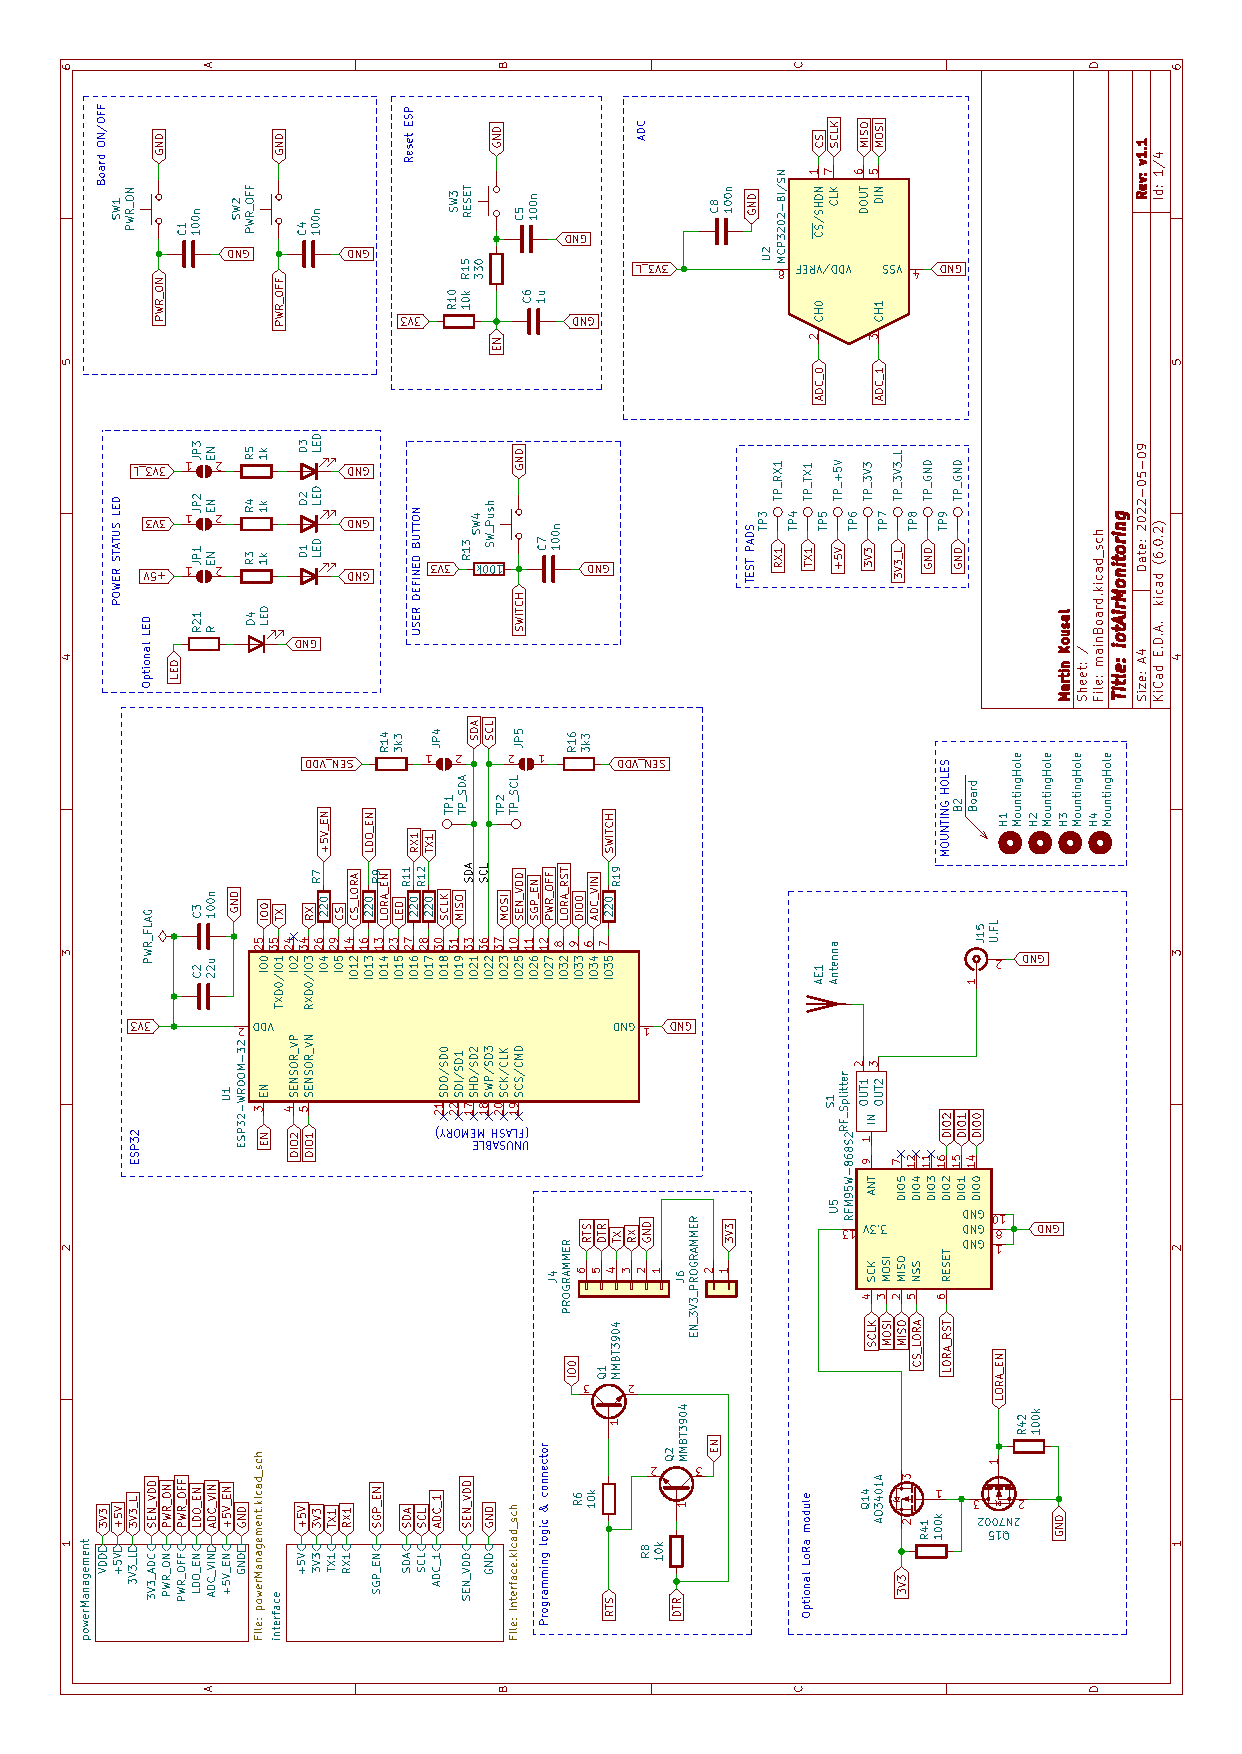
\includepdf[pages=1-]{obrazky/mainBoard.pdf}
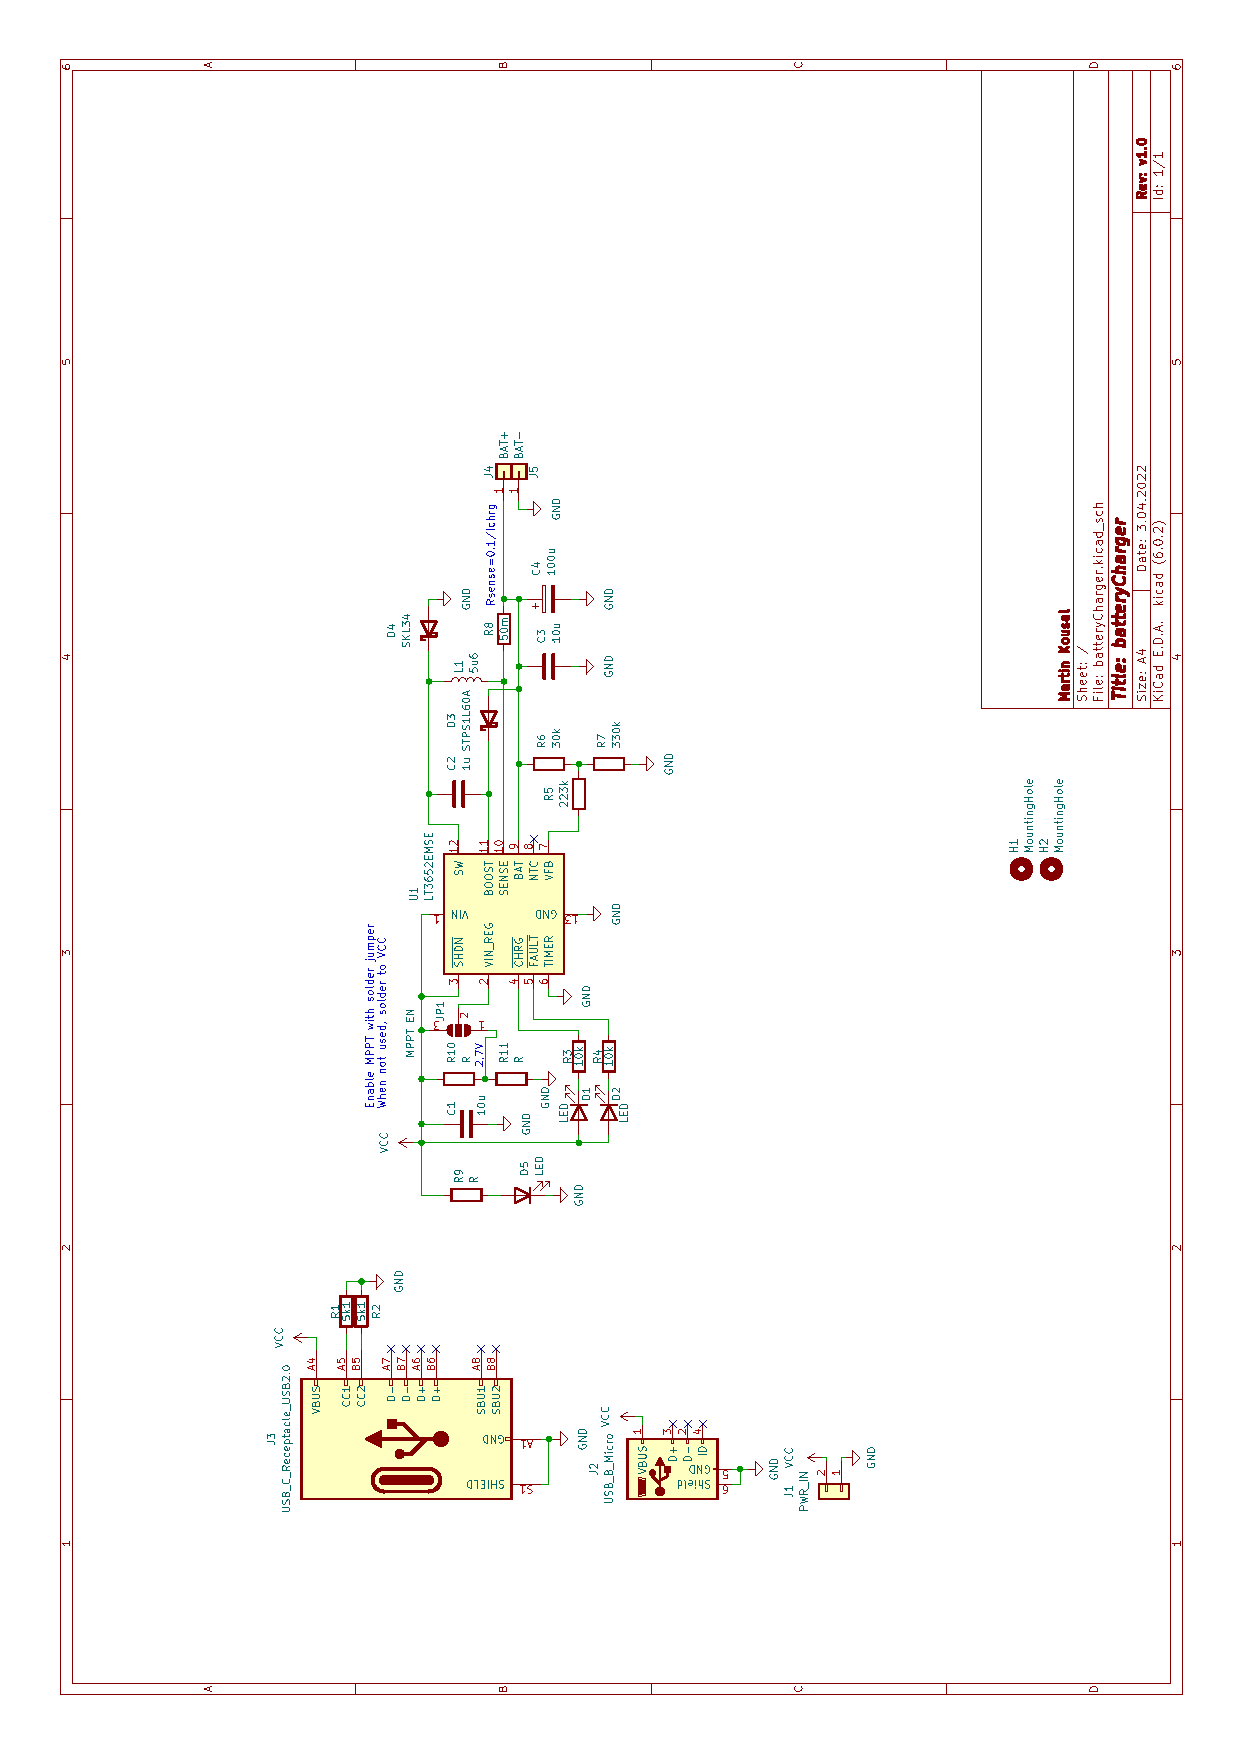
\includepdf[pages=1-]{obrazky/batteryCharger.pdf}

\chapter{Foto realizované desky plošných spojů}
\begin{figure}[h]
	\centering
	\subfloat[][Horní strana desky]{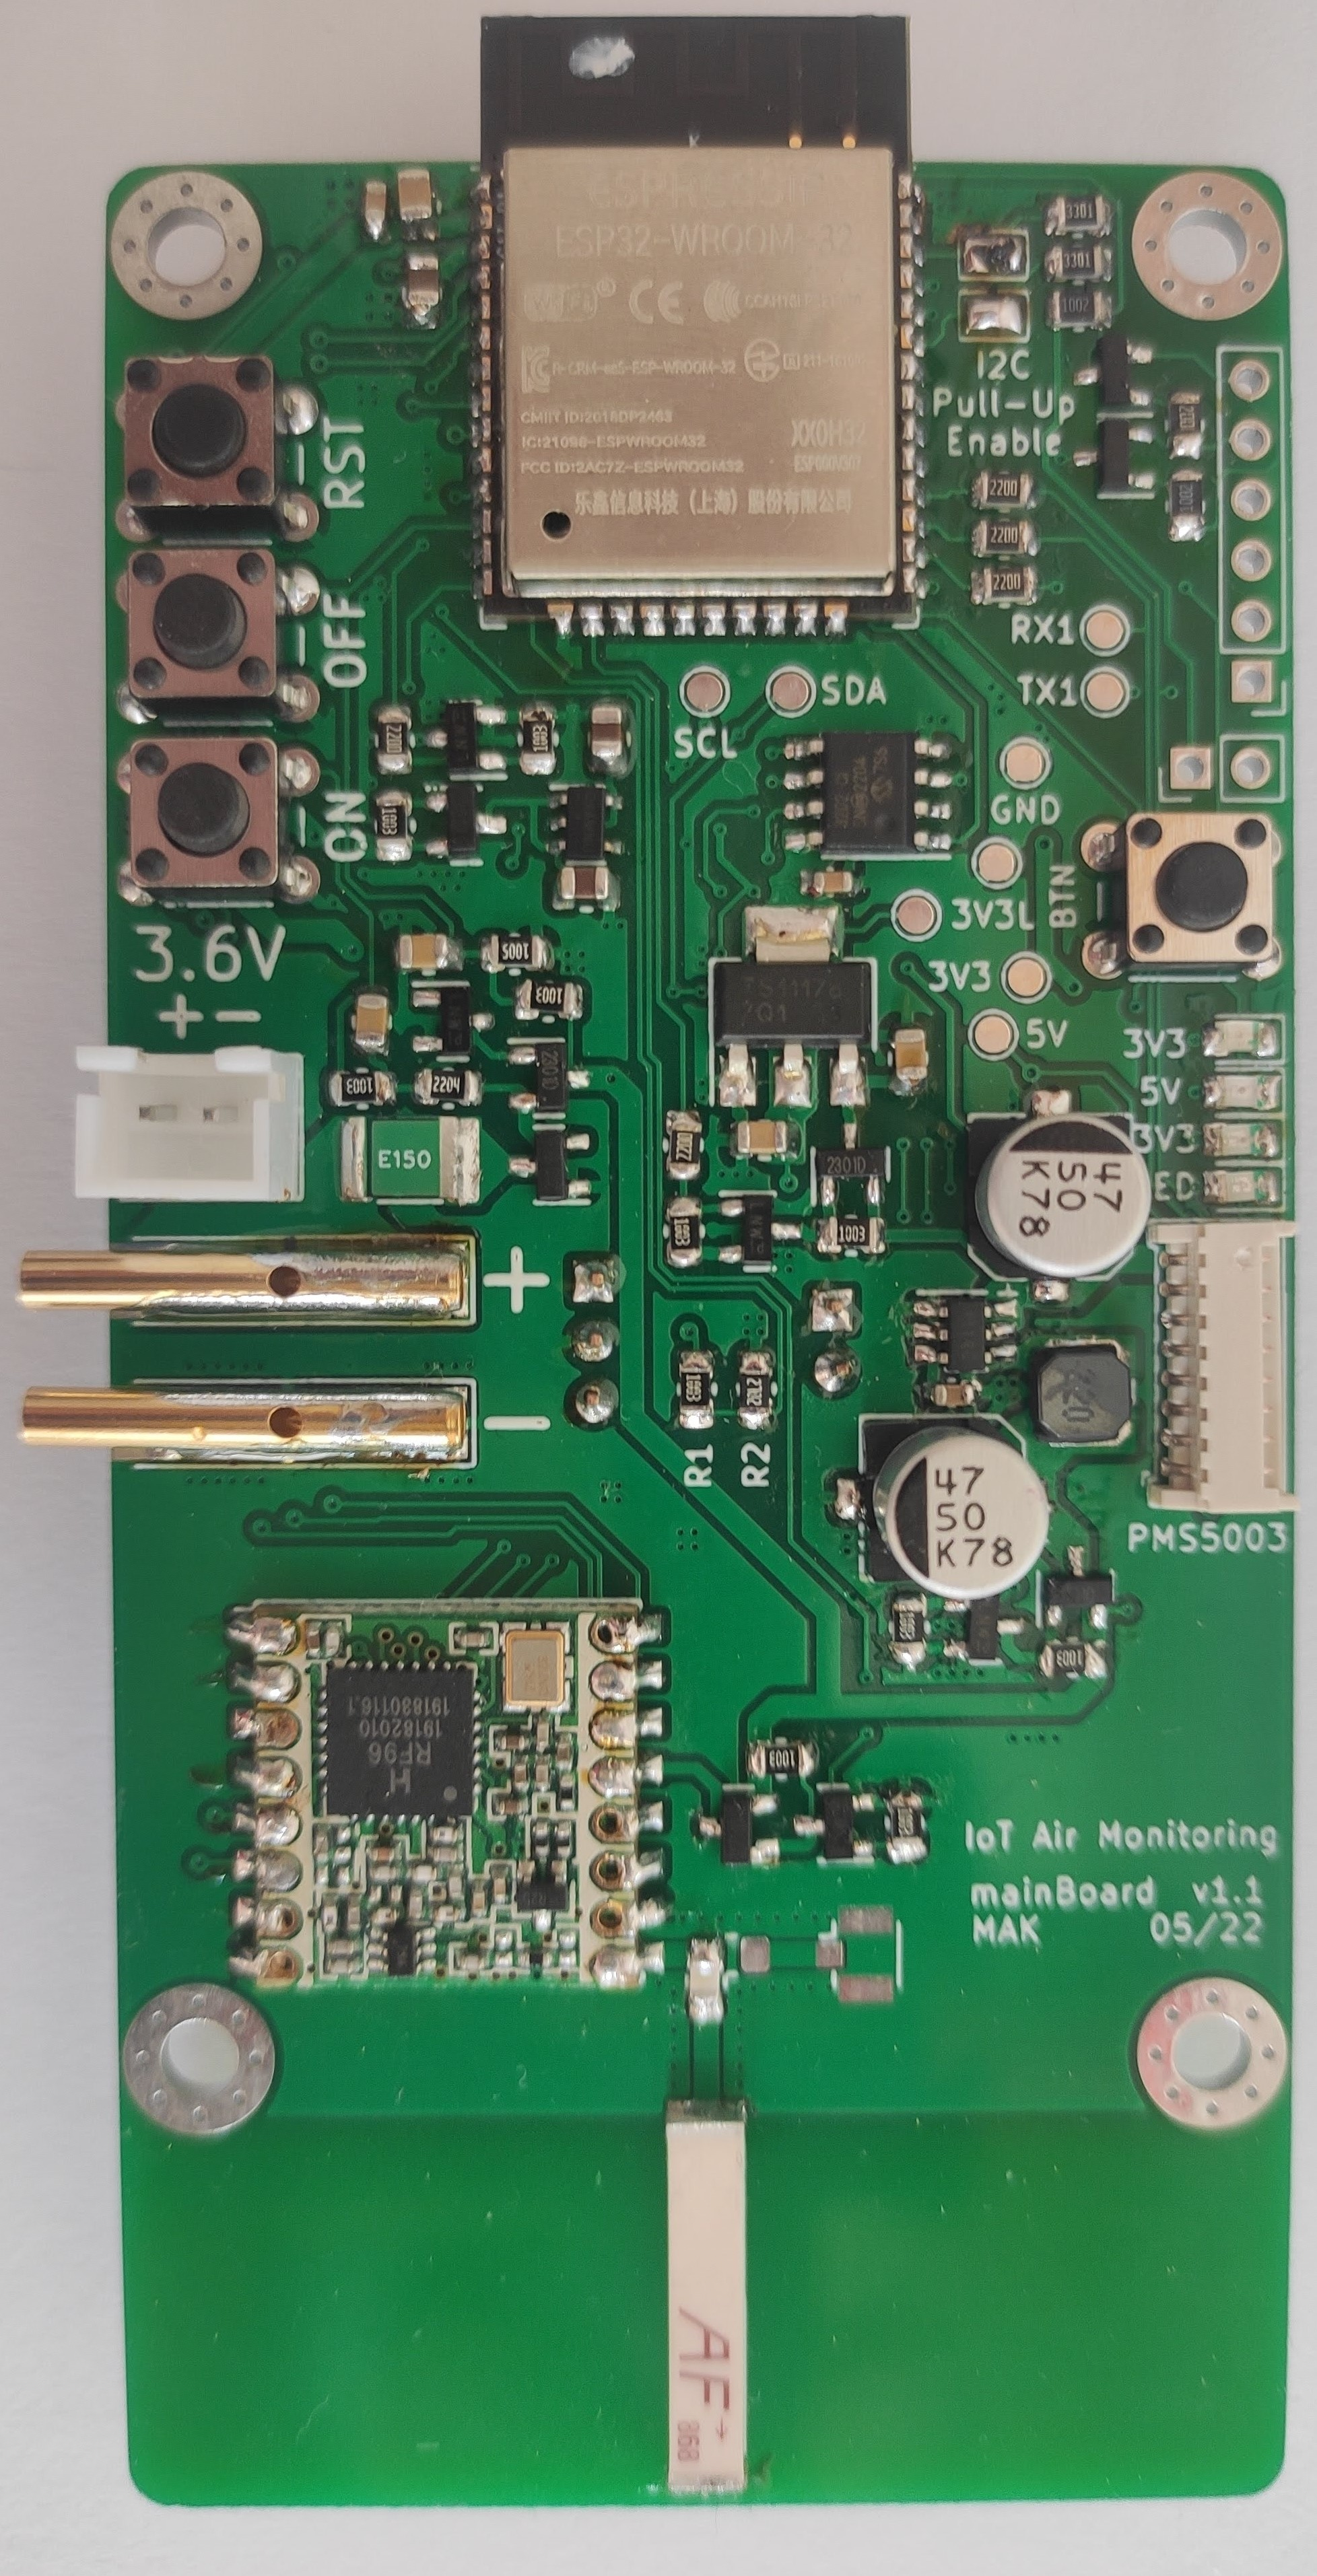
\includegraphics[width=0.48\textwidth]{obrazky/final_pcb_top.jpg}}
	\quad
	\subfloat[][Spodní strana desky]{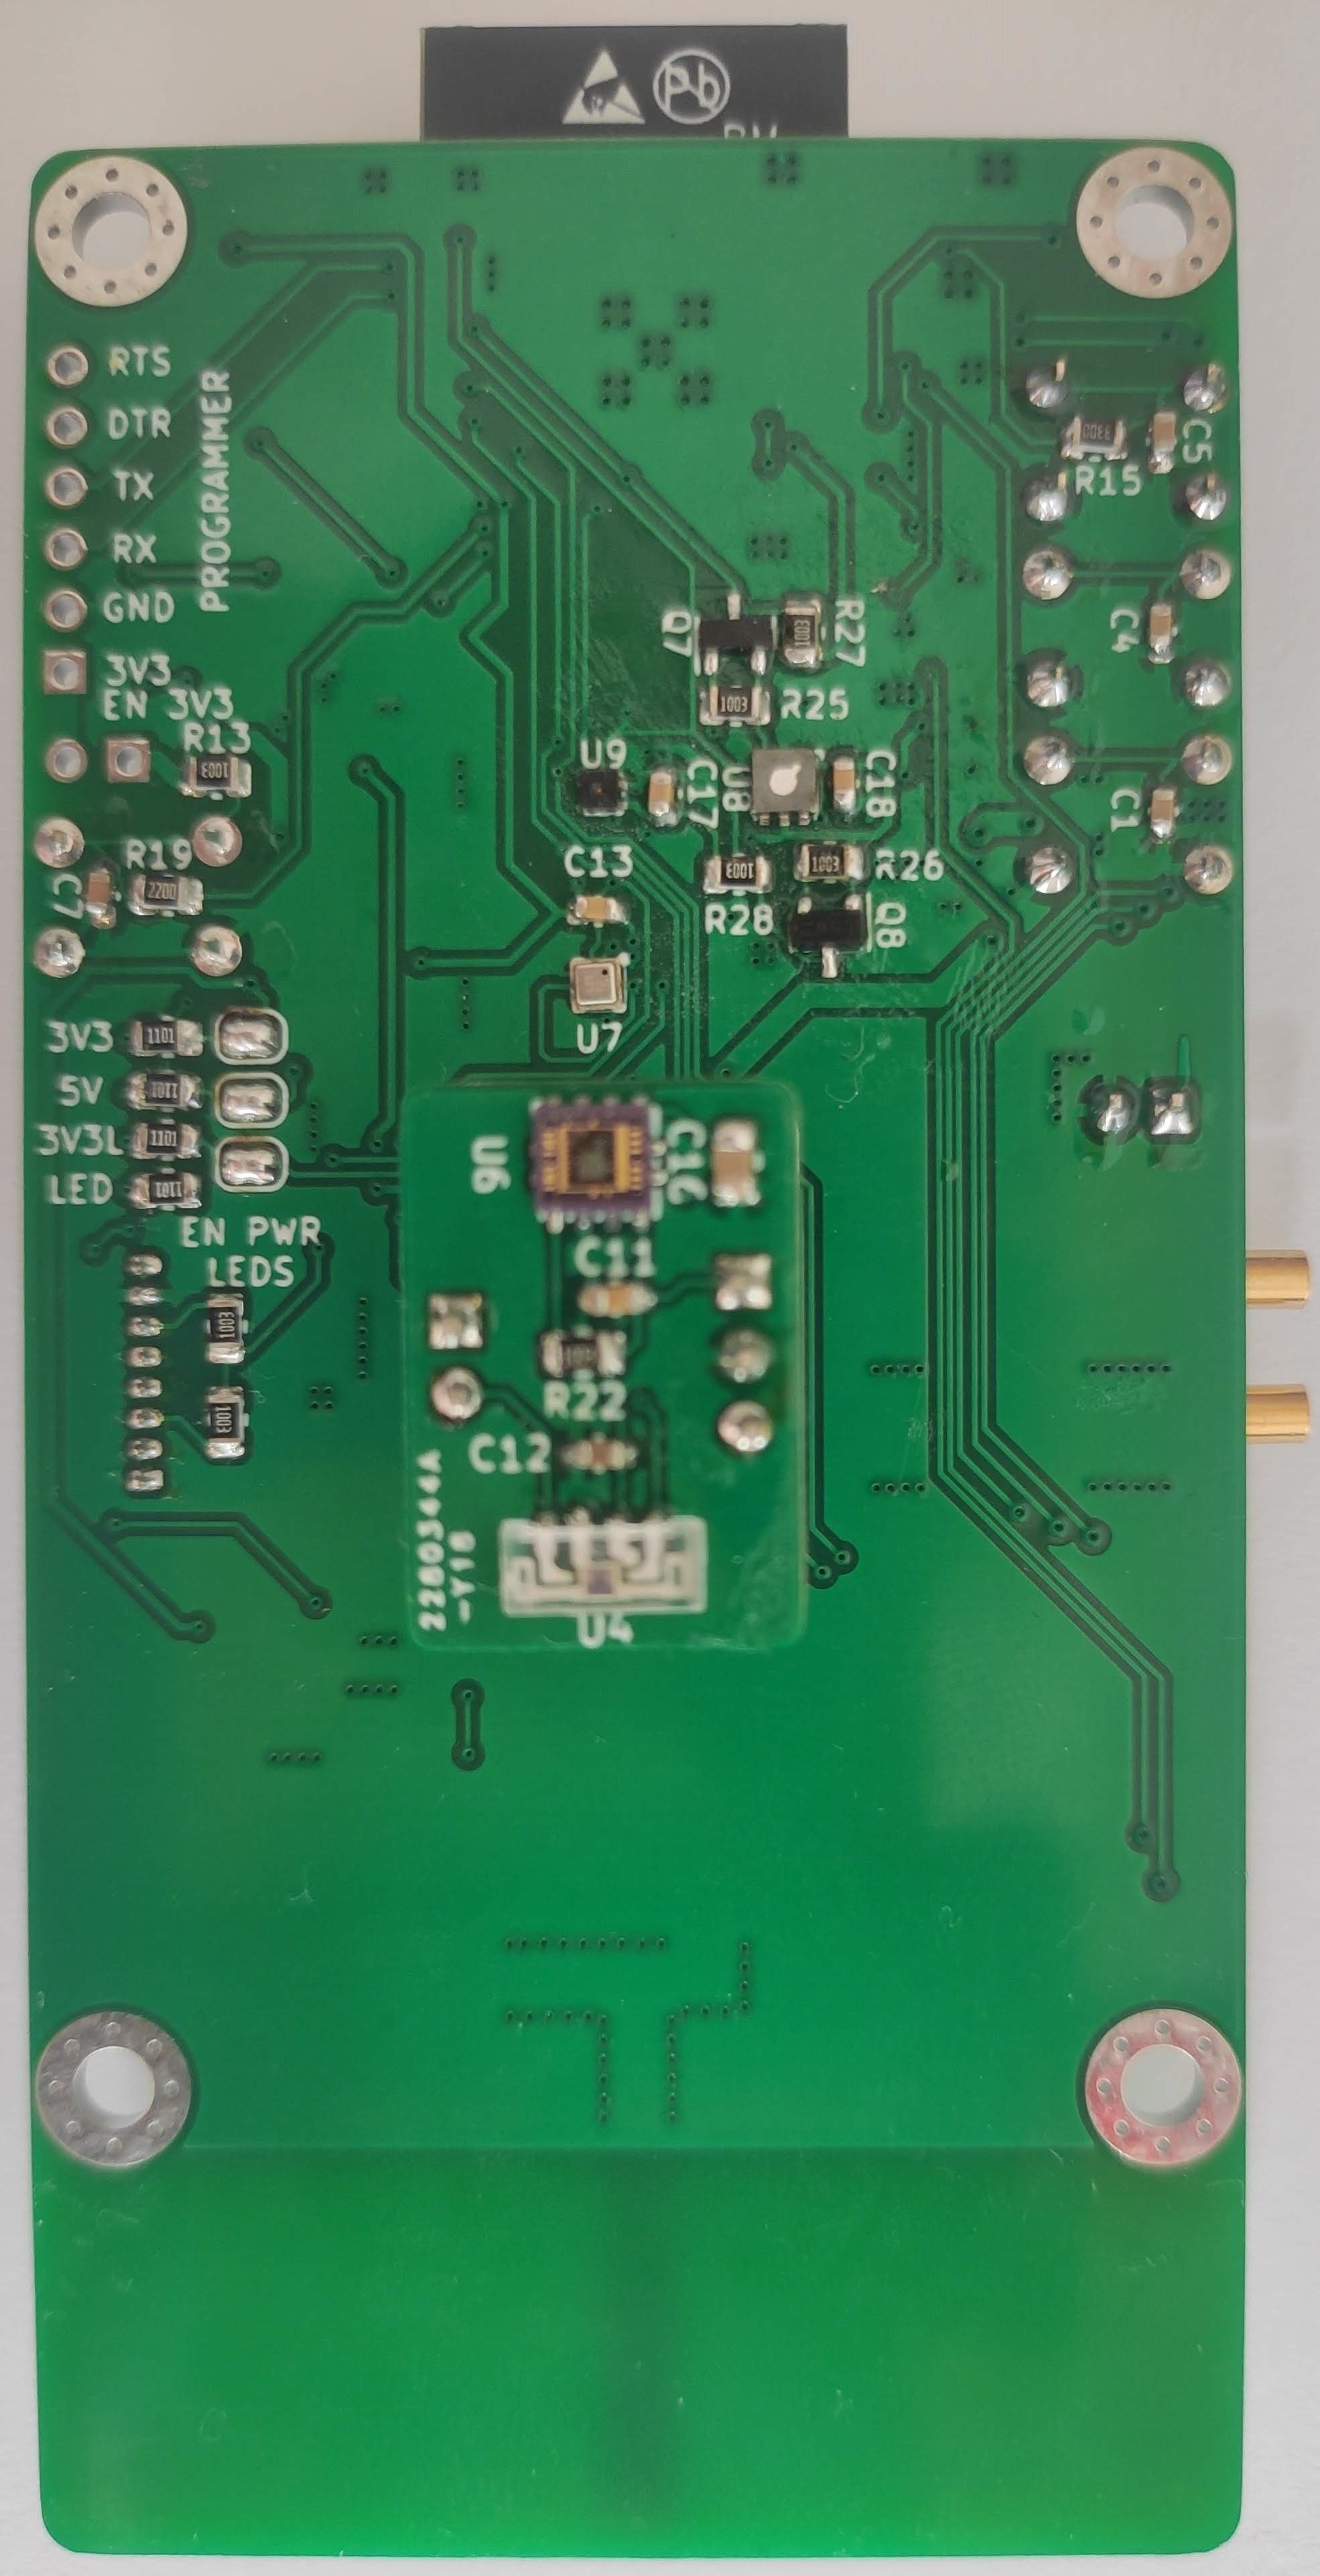
\includegraphics[width=0.48\textwidth]{obrazky/final_pcb_bot.jpg}}
	\caption{Foto osazené desky s~elektronikou včetně modulu světelných senzorů.}
	\label{fig_finalPCB}
\end{figure}

\chapter{Foto realizovaného zařízení}
\begin{figure}[h]
    \centering
    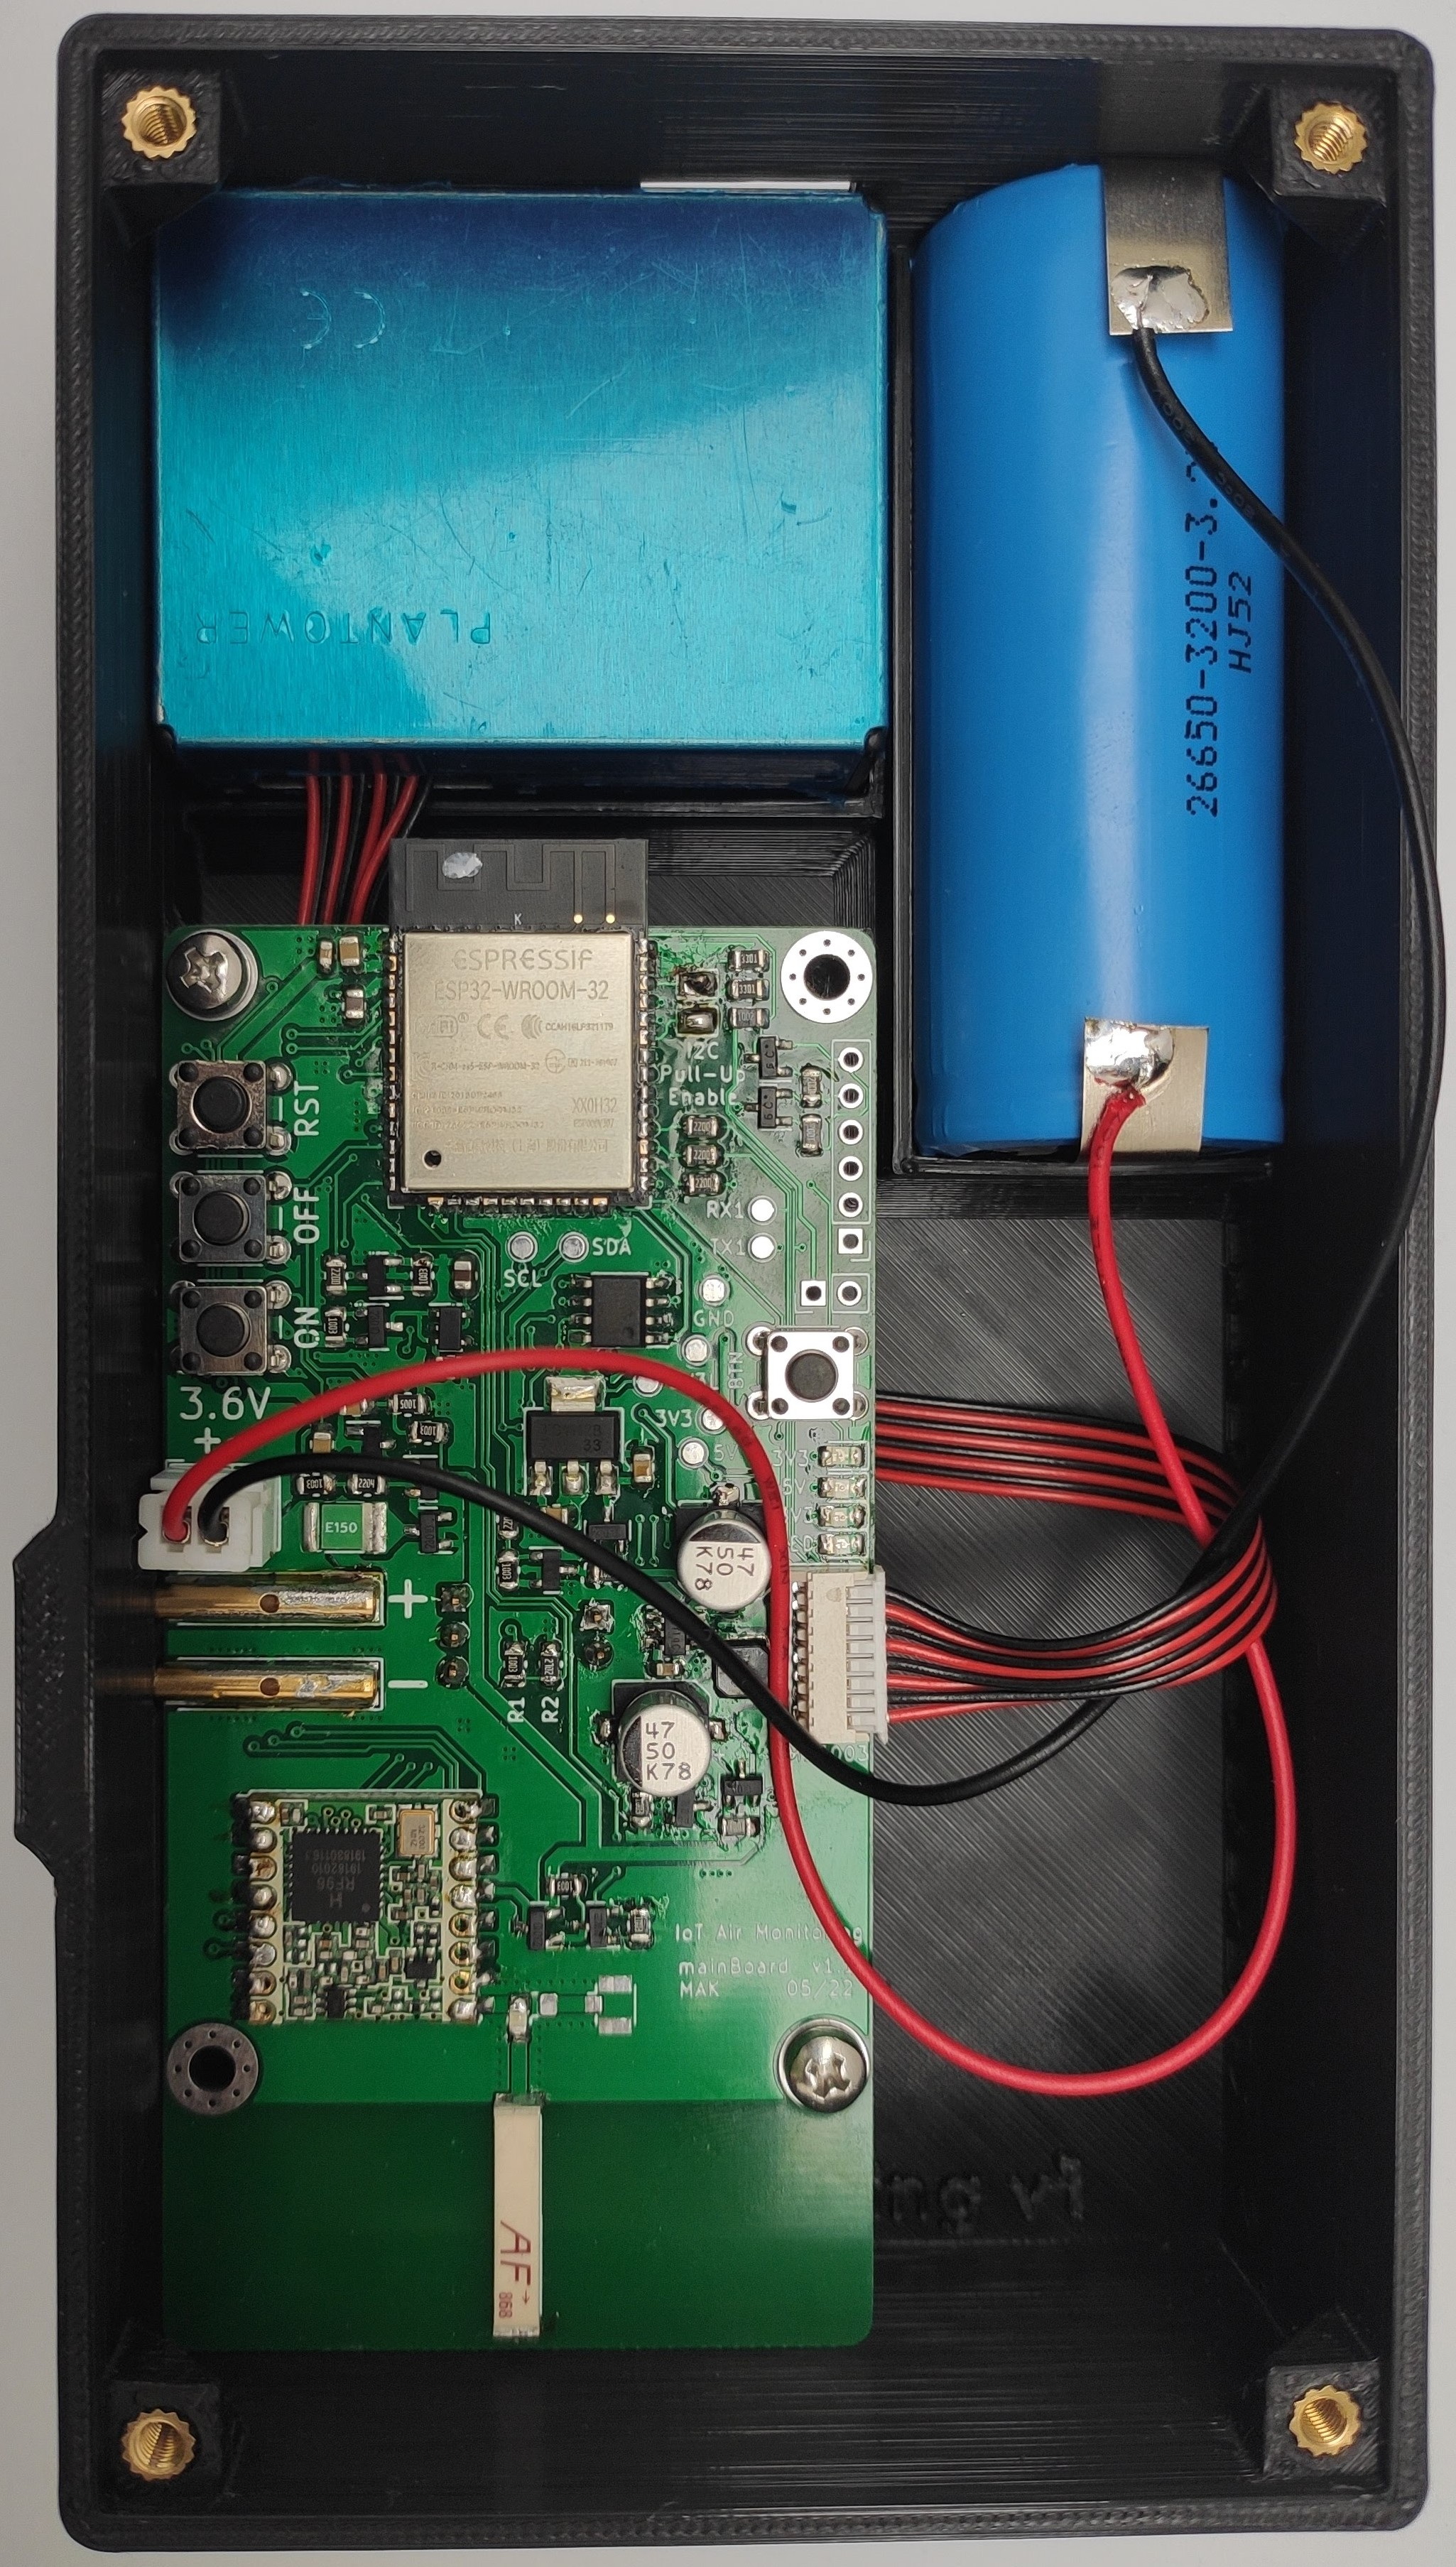
\includegraphics[height=0.7\textheight]{obrazky/finalDevice.jpg}
    \caption{Foto realizovaného zařízení v~krabičce.}
    \label{fig_finalDevice}
\end{figure}

\chapter{Obsah elektronické přílohy}

{\small
\dirtree{%
.1 /\DTcomment{Kořenový adresář přiloženého archivu}.
.2 hw\DTcomment{Podklady pro PCB}.
.3 mainBoard\DTcomment{Hlavní řídící deska a~modul světelných senzorů}.
.4 mainBoard.kicad_pro.
.4 mainBoard.kicad_sch.
.4 interface.kicad_sch.
.4 light_sensors.kicad_sch.
.4 powerManagement.kicad_sch.
.4 mainBoard.kicad_pcb.
.4 bom.pdf\DTcomment{Rozpiska součástek}.
.4 gerber\DTcomment{Výrobní podklady desek v~Gerber formátu}.
.5 gerber_mainBoard.zip.
.5 gerber_lightSensors.zip.
.3 batteryCharger\DTcomment{Deska nabíječky}.
.4 batteryCharger.kicad_pro.
.4 batteryCharger.kicad_sch.
.4 batteryCharger.kicad_brd.
.4 bom.pdf\DTcomment{Rozpiska součástek}.
.4 gerber.zip\DTcomment{Výrobní data v~Gerber formátu}.
.2 fw\DTcomment{Soubory pro firmware mikrokontroleru}.
.2 mec\DTcomment{Soubory s~3D modely krabičky}.
.3 case_bot.SLDPRT.
.3 case_top.SLDPRT.
.3 case_bot.stl.
.3 case_top.stl.
}
}

\end{document}